\documentclass[table]{beamer}
%\documentclass[table,handout]{beamer}
\usepackage{pgfpages}
%\setbeameroption{show notes}
%\setbeameroption{show only notes}
%\setbeameroption{show notes on second screen=left}
\usepackage{listings}
\usepackage{multirow}
\usepackage{natbib}
\usetheme[secheader]{Madrid}
%\usepackage[francais]{babel}
%\usepackage[utf8]{inputenc}
\usepackage{subfigure}
\usepackage{amsmath}
\usepackage{multimedia}
\usepackage{tipa}
\usepackage{comment}
\usepackage[official]{eurosym}
\usepackage{url}
\usepackage{hyperref}
\usepackage{multimedia}
\usepackage{amssymb}

%\movie[showcontrols,poster,width=4cm,height=2cm]{video}{recording_Basaa.mp4}
%\usepackage{movie15}
%\usepackage[cjkjis]{ucs}
%\usepackage[utf8]{inputenc}
%\usepackage[C42,T1]{fontenc}
%\DeclareFontSubstitution{C42}{dg}{m}{n}


\usepackage{xcolor}
\usepackage{colortbl}
\definecolor{LigAikumaGreen}{RGB}{15,151,0}
\definecolor{LigAikumaRed}{RGB}{202,11,0}

\usepackage{fontawesome}
\newcommand{\facheckmark}{\textcolor{LigAikumaGreen}{\faCheck}}
\newcommand{\facrossmark}{\textcolor{LigAikumaRed}{\faClose}}
\newcommand{\faRedMinusCircle}{\textcolor{LigAikumaRed}{\faMinusCircle}}
\newcommand{\faGreenPlusCircle}{\textcolor{LigAikumaGreen}{\faPlusCircle}}
\newcommand{\faBluePlusCircle}{\textcolor{blue}{\faPlusCircle}}
\newcommand{\faGreenCheck}{\textcolor{LigAikumaGreen}{\faCheckSquareO}}
\newcommand{\faOrangeCogs}{\textcolor{orange}{\faCogs}}
\newcommand{\faColoredLaptop}{\textcolor{fire}{\faLaptop}}
\newcommand{\faColoredLanguage}{\textcolor{grass}{\faLanguage}}


\usepackage{multirow}
\usepackage{tabularx}
\usepackage{graphicx}
\usepackage{tipa}
\usepackage[autolanguage]{numprint}
\usepackage{tcolorbox}
\usepackage{xifthen}
\usepackage{fontawesome}

\usepackage{ragged2e} %text alignment
\usepackage{ulem} %strike out
\newcommand\redout{\bgroup\markoverwith
{\textcolor{red}{\rule[0.5ex]{2pt}{0.8pt}}}\ULon}

%\newcommand{\facheckmark}{\textcolor{LigAikumaGreen}{\faCheck}}
%\newcommand{\facrossmark}{\textcolor{LigAikumaRed}{\faClose}}
%\newcommand{\faRedMinusCircle}{\textcolor{LigAikumaRed}{\faMinusCircle}}
%\newcommand{\faGreenPlusCircle}{\textcolor{LigAikumaGreen}{\faPlusCircle}}
%\newcommand{\faBluePlusCircle}{\textcolor{blue}{\faPlusCircle}}
%\newcommand{\faGreenCheck}{\textcolor{LigAikumaGreen}{\faCheckSquareO}}
%\newcommand{\faOrangeCogs}{\textcolor{orange}{\faCogs}}
%\newcommand{\faColoredLaptop}{\textcolor{fire}{\faLaptop}}
%\newcommand{\faColoredLanguage}{\textcolor{grass}{\faLanguage}}
%



%\usefonttheme{professionalfonts}
%\usepackage{txfonts}
%\usepackage{tikz}
%\usetikzlibrary{arrows}
%\usetikzlibrary{shapes}

\usepackage{color}
\usepackage{colortbl}%\DeclareGraphicsExtensions{.jpg,.mps,.pdf,.png}

\newcommand{\bulb}{{\sc Bulb}}
\newcommand{\aikuma}{{\sc Aikuma}}
\newcommand{\ligaikuma}{{\sc Lig-Aikuma}}
\newcommand{\android}{Android}

\newcommand{\bulbBold}{{\sc \textbf{Bulb}}}
\newcommand{\aikumaBold}{{\sc \textbf{Aikuma}}}
\newcommand{\ligaikumaBold}{{\sc \textbf{Lig-Aikuma}}}
\newcommand{\androidBold}{\textbf{Android}}

\usepackage{bm}
\setbeamertemplate{bibliography item}[text]


\definecolor{blue}{rgb}{0.5,0.5,0.7}
\definecolor{lblue}{rgb}{0.8,0.8,1.0}


\def\colbox#1#2{{
\noindent \fcolorbox{blue}{lblue}{
\begin{minipage}{0.95\textwidth}
\begin{center}
{{\bf #1}}\hspace*{0.2cm} {\bf #2}
\end{center}
%\vspace*{-0.02cm}
\end{minipage}}
}}


\title[SelfSupSpeech]{Self Supervised Representation Learning from Speech}
%\subtitle{Une brève histoire de la reconnaissance de la parole \\ (mais qui commencerait seulement dans les année 90 ...)}
%\author[L. Besacier]{\textbf{Laurent Besacier}, Elodie Gauthier, Sylvie Voisin \vspace*{0.1cm}}
\author[L. Besacier]{\textbf{Laurent Besacier} }
\institute[LIG]{
\includegraphics[height=2cm]{LIG_coul}%\hspace*{1cm}

%In this talk i will describe the task of automatic speech recognition (ASR) and the evolution of the approaches proposed over the last decades. I will also present current trends (such as end-to-end ASR) and open problems (such as low resource conditions) that remain to be addressed in this domain.
}
\date[June 16th 2020]{}%{date longue : document révisé le \today}

\begin{document}
\frame{\maketitle}


\begin{frame}{Outline}
	\tableofcontents
\end{frame}



%\frame{\tableofcontents[currentsection]}

%%%INTRO
\section{Introduction}

\begin{frame}
\frametitle{Self supervised representation learning}
\begin{itemize}
	\item Using huge unlabeled data for training ; targets are computed from the signal itself
		\begin{itemize}
		\item \textit{''learn representations using objective functions similar to those used for supervised learning, but train networks to perform pretext tasks where both the inputs and labels are derived from an unlabeled dataset''} (from \cite{norouzi} )
		\end{itemize}
	\item Introduced for vision: see for instance  \citep{norouzi} 
	\begin{itemize}
		\item learn representations by contrasting positive pairs against negative pairs
	\end{itemize}
	\item Introduced also in NLP: see for instance \citep{bert}
	\begin{itemize}
		\item more details in next slides  
	\end{itemize}
\end{itemize}

\end{frame}


%%%INTRO

\begin{frame}
\frametitle{Previous works}
\begin{itemize}
	\item Stacked restricted Boltzman machines (RBM) \citep{HinSal06}
		\begin{itemize}
		\item hidden layer extracts relevant features from the observations that serve as input to next RBM that is stacked on top of it forming a deterministic feed-forward neural network
		\end{itemize}
	\item Denoising autoencoders (AE) \citep{Vincent08extractingand}
		\begin{itemize}
		\item networks which are tasked with reconstructing outputs from their (noisy) input versions
		\end{itemize}
	\item Variational autoencoders (VAE) \citep{kingma2013autoencoding}
		\begin{itemize}
		\item VAE is like a traditional AE in which the encoder produces distributions over latent representations (rather than deterministic encodings) while the decoder is trained on samples from this distribution
		\item both encoder and decoder are trained jointly
		\item VQ-VAE \citep{NIPS2017_7210} replaces continuous latent vectors with deterministically quantized versions
		\end{itemize}
\end{itemize}

\end{frame}



%%%%include here Hang Le's slides !!!!
\begin{frame}
\frametitle{Pre-trained language models}
	\begin{itemize}
		\item Leverage large amount of freely available unlabeled text to facilitate transfer learning in NLP
		\item Yield state-of-the-art results on a wide range of NLP tasks + save time and computational resources
		\item Example of BERT \citep{bert} based on the Transformer model \citep{Vaswani2017}
	\end{itemize}
	
	\begin{center}
	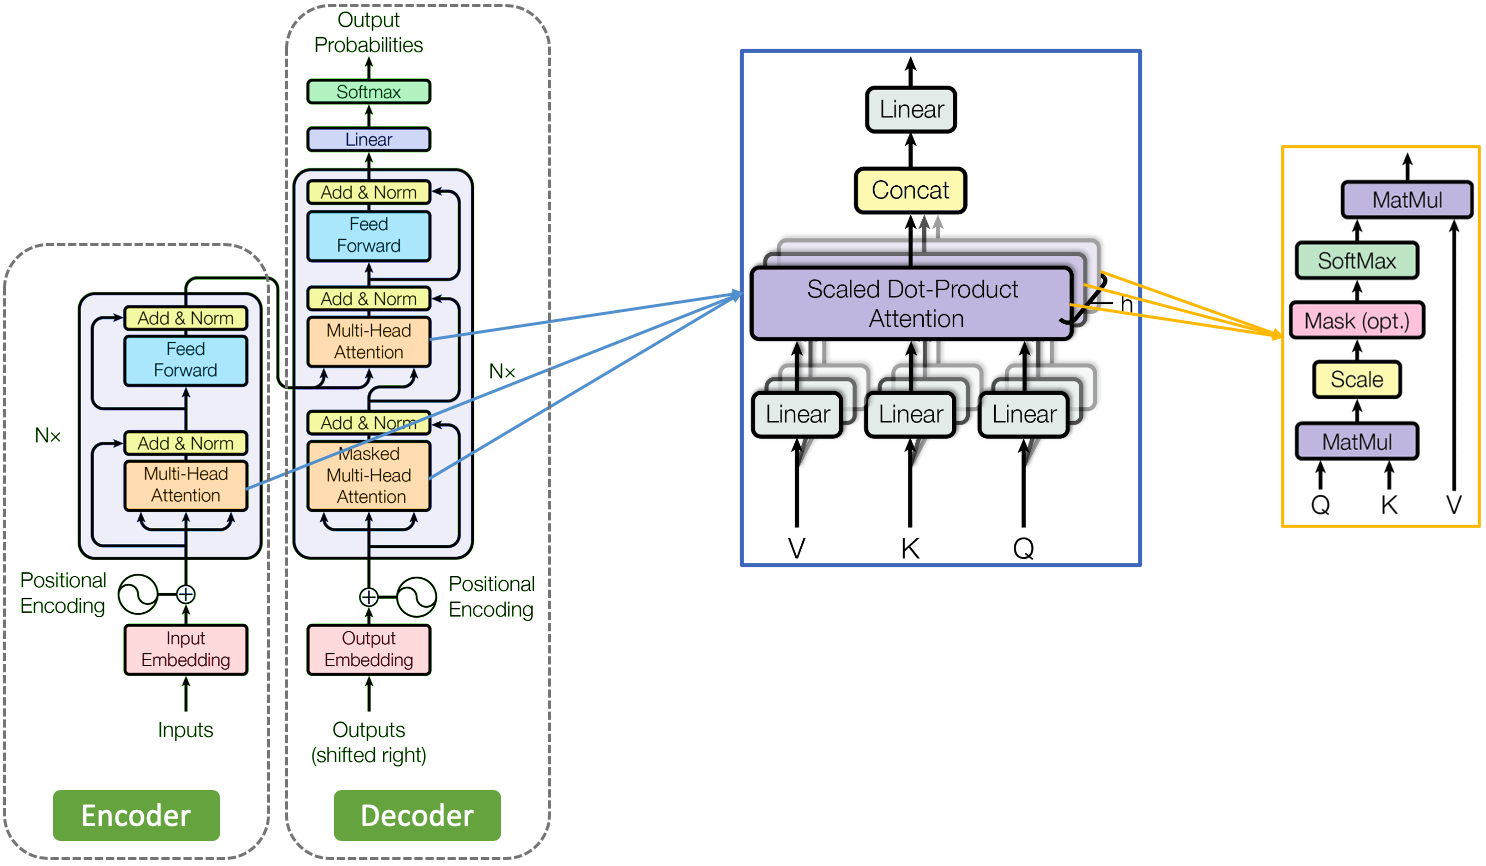
\includegraphics[width=0.81\textwidth]{transformer_all}
	\end{center}


\end{frame}


\begin{frame}{Pre-training: example of BERT}{}	
Following the BERT~\cite{bert} paradigm
\begin{center}
	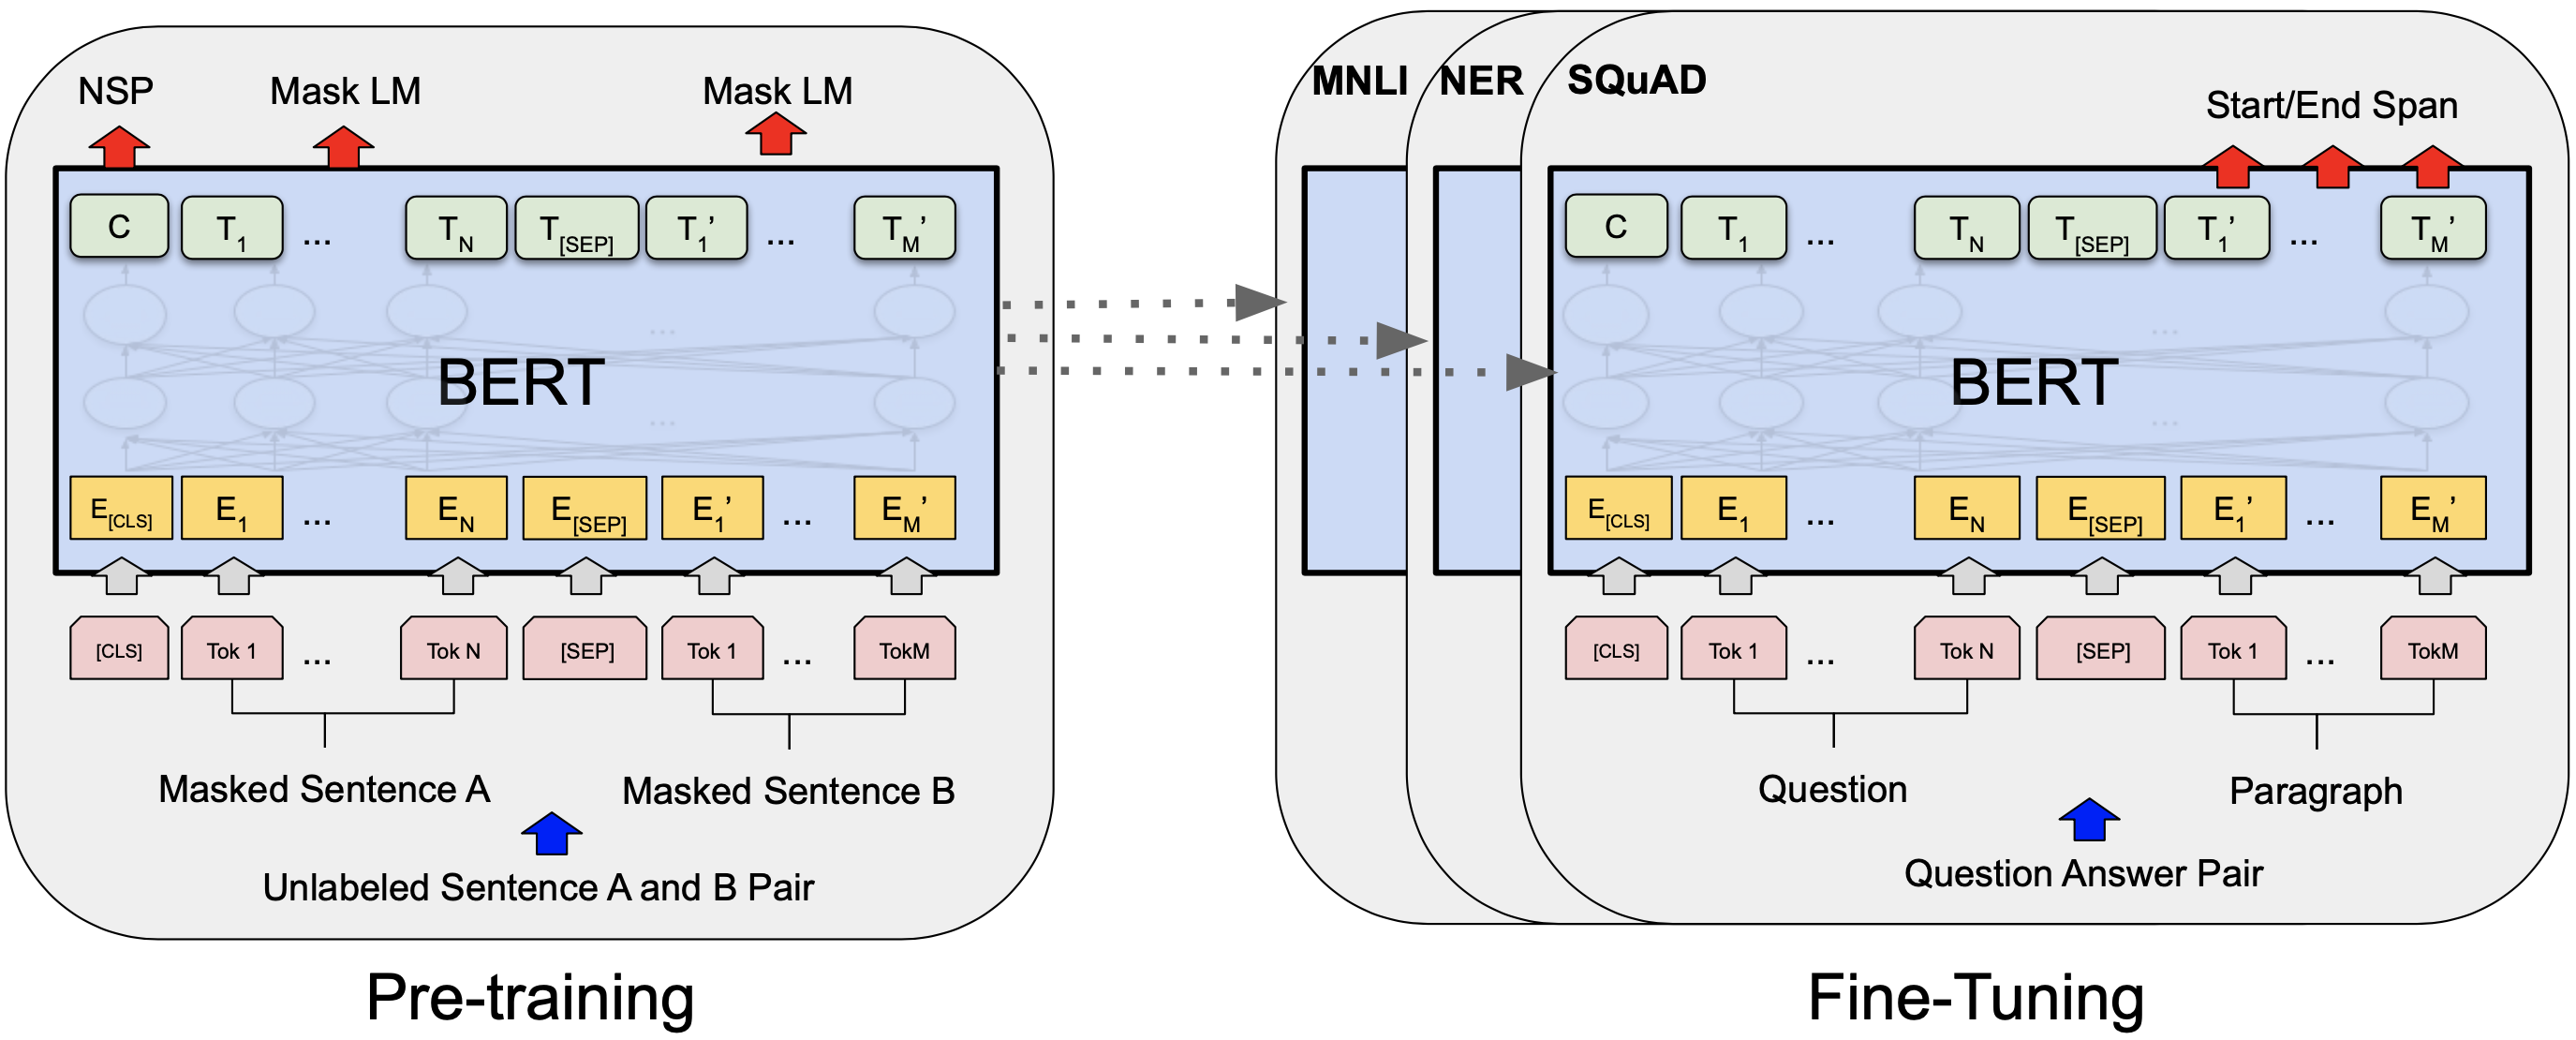
\includegraphics[width=0.8\textwidth]{bert_finetune}
\end{center}
	\begin{itemize}
		\item \textbf{Masked Language Model}: learn to predict randomly masked input tokens.
		\item \textbf{Next Sentence Prediction}: learn to predict if $B$ is the next sentence to $A$, given an input pair $(A,B)$. 
	\end{itemize}

\end{frame}



%%%%%%%%%%%


%%%SPEECH


%%%%%%%


\begin{frame}
\frametitle{Self supervised representation learning from speech}
\begin{itemize}
	\item Autoregressive predictive coding (APC) \citep{DBLP:journals/corr/abs-1904-03240,chung2020improved}
		\begin{itemize}
		\item Considers the sequential structure of speech and predicts information about a future frame
		\end{itemize}
	\item Contrastive Predictive Coding (CPC) \citep{Baevski, Schneider2019,morgane}
		\begin{itemize}
		\item Easier learning objective which consists in distinguishing a true future audio frame from negatives
		\end{itemize}	
	\item Other approaches for feature representation learning using multiple self supervised tasks \citep{pascual2019,ravanelli2020multitask} or bidirectional encoders \citep{song2019speechxlnet,Liu_2020, wang2020unsupervised}
\end{itemize} 
\end{frame}



%%%%%%%



%%%%%%%
\section{Autoregressive predictive coding (APC)}

\begin{frame}
\frametitle{Autoregressive predictive coding (APC)}
\begin{itemize}
\item Predicting the spectrum of a future frame (rather than a wave sample)
\item Largely inspired by language models (LMs) for text, which are typically a probability distribution over sequences of T tokens $(t_1,t_2,...,t_T )$
\begin{equation}
	P(sequence) = \prod_{k=1}^{T} P(t{_{k}}|t{_{1}},t{_{2}},...,t{_{k-1}})
\end{equation}
\begin{equation}
	P(sequence) = \prod_{k=1}^{T} P(t{_{k}}|h)
\end{equation}
\item Recurrent neural network LM: $h=rnn\_state(E(t{_{1}}),E(t{_{2}}),...,E(t{_{k-1}}))$
\item For speech, each token $t_k$ corresponds to a frame rather than a word or character token
\end{itemize} 
\end{frame}


%%%%%%%

\begin{frame}
\frametitle{Autoregressive predictive coding (APC)}
\begin{itemize}
\item Differences between speech and text tokens
		\begin{itemize}
			\item Input speech representations (MFCCs for instance) are already in a vector form (no embedding layer)
			\item No final set of target tokens (softmax layer replaced by a regression layer)
			\item Learnable parameters in APC are the RNN parameters $\theta_{rnn}$ and the regression layer parameters $\theta_r$
			\item Encourage APC to infer more global structures rather than the local information in the signal
				\begin{itemize}
				\item ask the model to predict a frame $n$ steps ahead of the current one
				\end{itemize}
			\item Model is optimized by minimizing the L1 loss between input sequence $(t_1,t_2,...,t_T )$ and the predicted sequence $(y_1,y_2,...,y_T )$:
				\begin{equation}
				\sum_{i=1}^{T-n} | t_i-y_i |,t_i=x_{i+n}
				\end{equation}			
		\end{itemize} 
\end{itemize} 
\end{frame}


%%%%%%%


\begin{frame}
\frametitle{Autoregressive predictive coding (APC)}
\begin{itemize}
\item  \cite{DBLP:journals/corr/abs-1904-03240} models APC with a multi-layer unidirectional LSTM with residual connections
\item After training, RNN hidden states are taken as the learned representations
\item A follow-up work \citep{chung2020improved} adds an auxiliary objective that serves as regularization to  improve generalization 
\end{itemize} 
\begin{figure}
	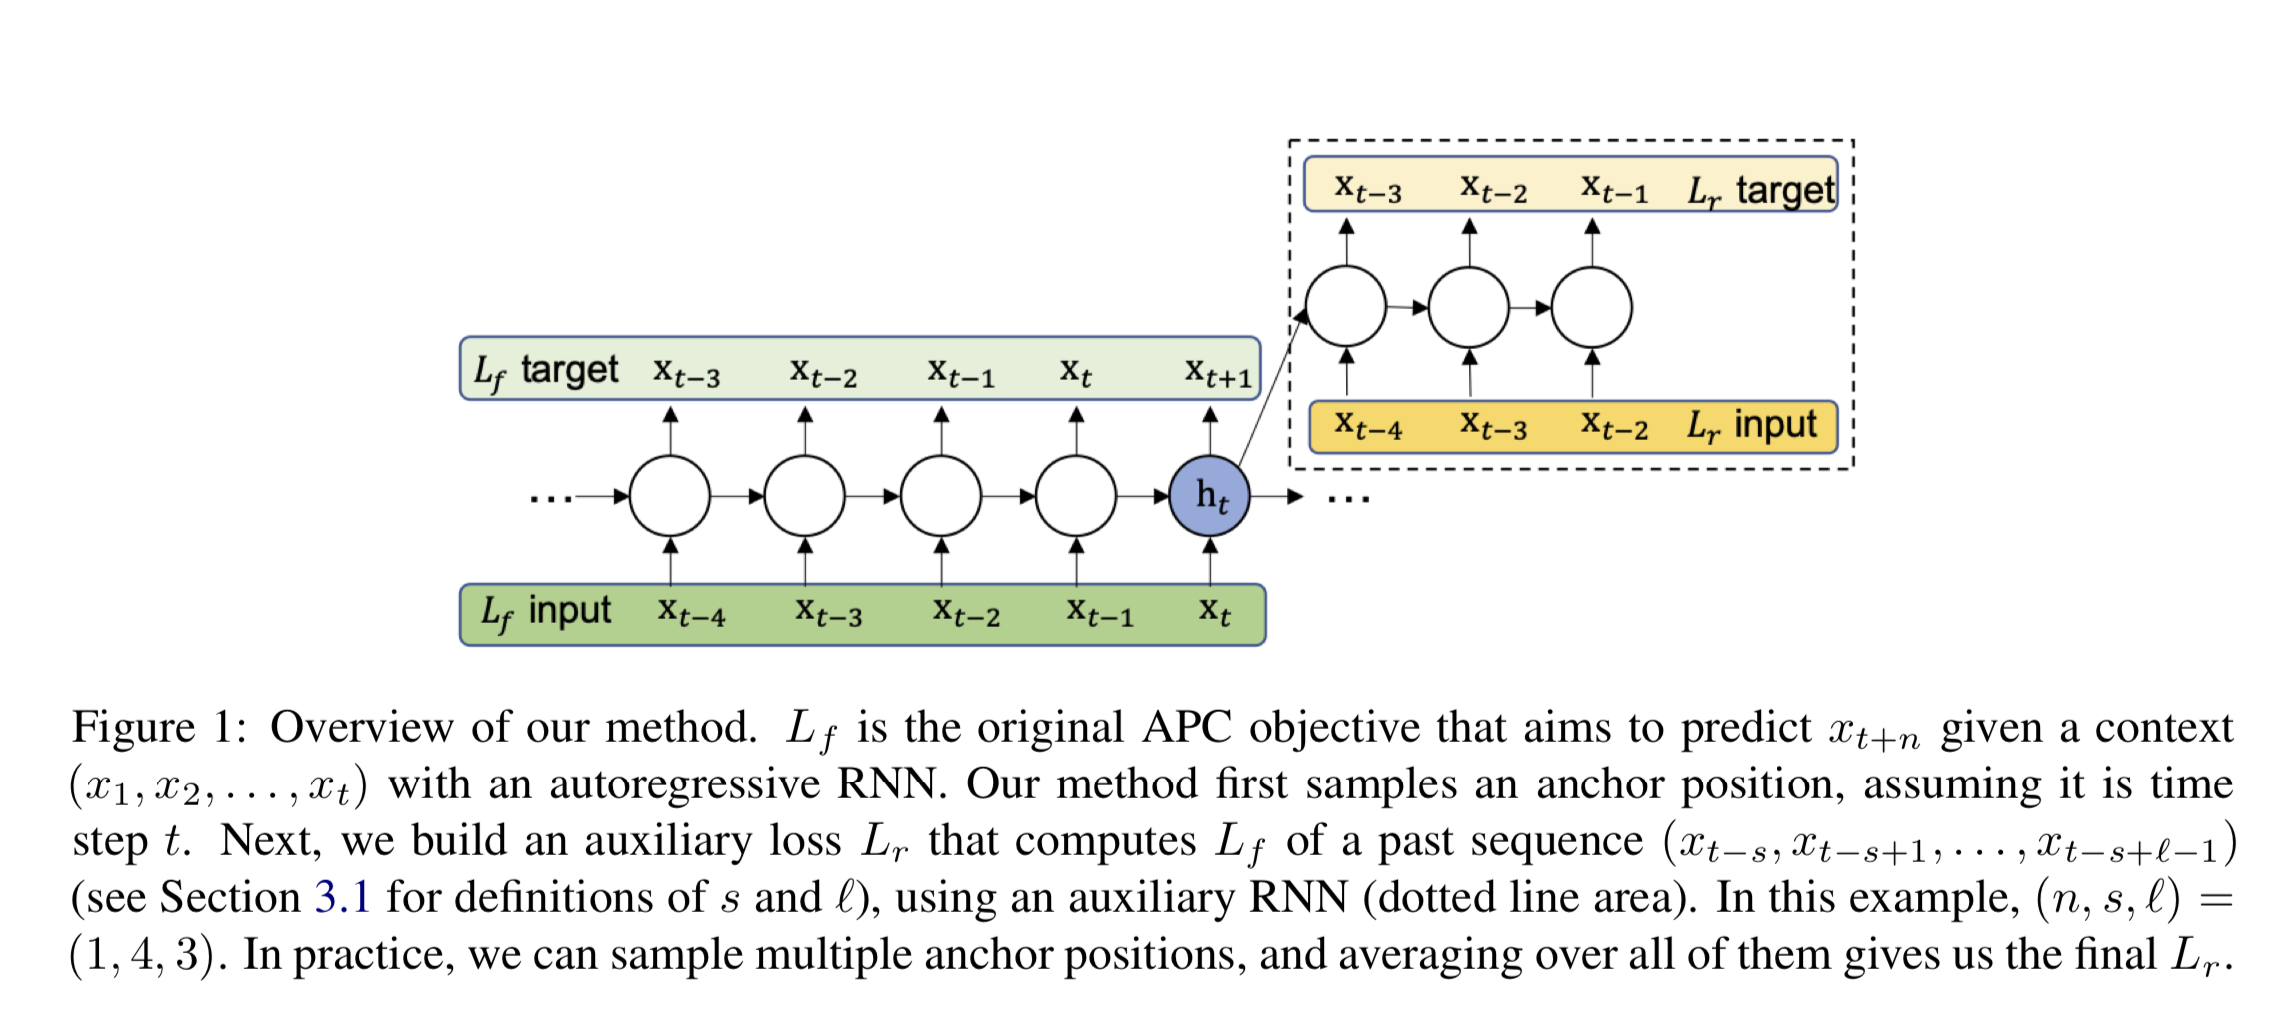
\includegraphics[width=0.65\textwidth]{regularization}
	\caption{Figure from  \citep{chung2020improved}}
\end{figure}

\end{frame}


%%%%%%%

\begin{frame}
\frametitle{Autoregressive predictive coding (APC)}
\begin{itemize}
\item Speech transcription and translation experiments on Librispeech
\item Architecture is a RNN model with attention
\end{itemize} 
\begin{center}
	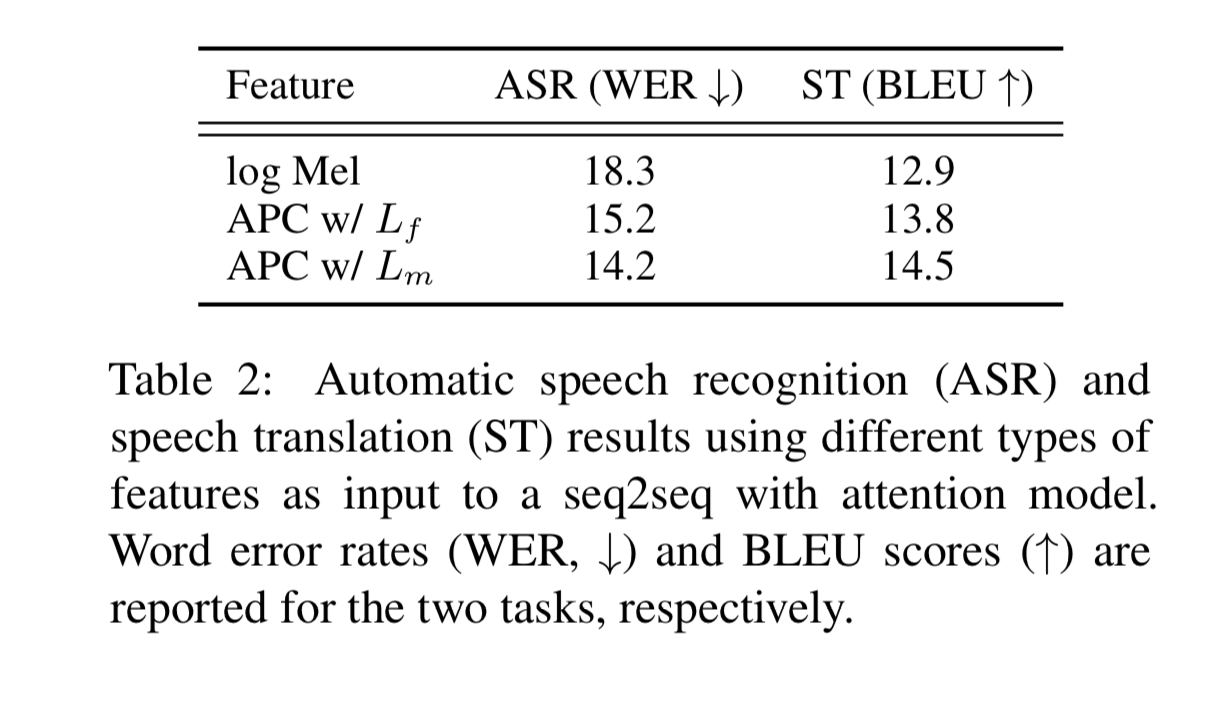
\includegraphics[width=0.8\textwidth]{APCexp}
\end{center}

\end{frame}



%%%%%%%%%%

\section{Contrastive predictive coding (CPC)}


\begin{frame}
	\frametitle{Contrastive Predictive Coding (CPC)}
		\begin{itemize}
			\item Use  of a contrastive loss that distinguishes a true future audio sample from negatives
			\item Example of \textit{wav2vec} \citep{DBLP:journals/corr/abs-1904-05862} that relies on a fully convolutional architecture
			\item Applied the learned representations to improve a supervised ASR system
		\end{itemize} 

		\begin{figure}
			\centering
			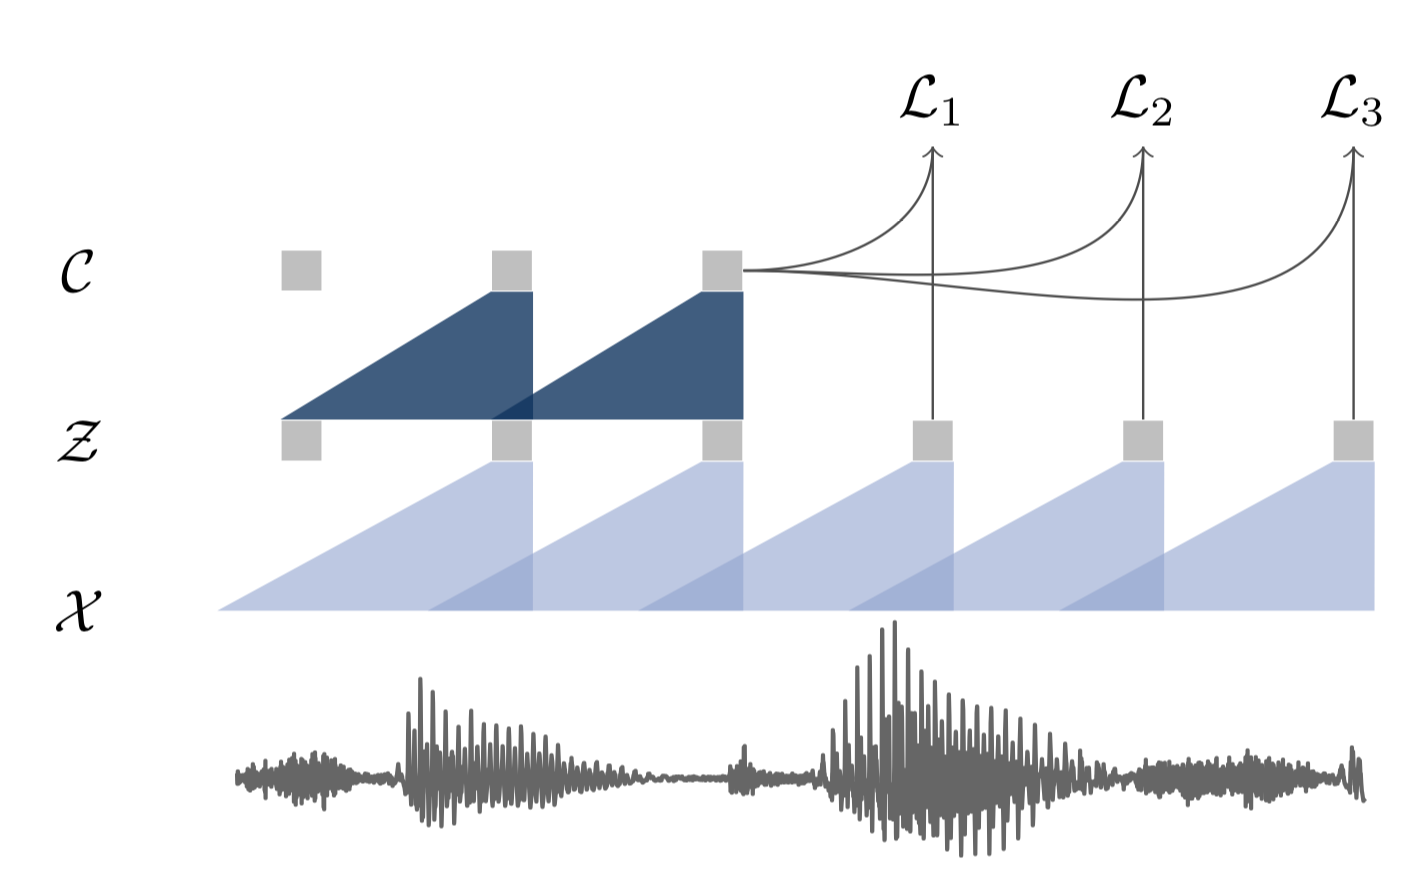
\includegraphics[scale=0.21]	{unsupervisedspeech.png} 
		%	[scale=0.35,trim=0mm 140mm 0mm 0mm,clip=true]
			\caption{Figure from \citep{DBLP:journals/corr/abs-1904-05862}}
			\label{fig:unsup}
			\end{figure}

	
\end{frame}


\begin{frame}
	\frametitle{Contrastive Predictive Coding (CPC)}
		\begin{itemize}
			\item Encoder network $Z=f(X)$ ; 5 (causal) convolution layers ; local feature representations $z_i$ encode 30 ms of audio every 10ms
			\item Context network $C=g(Z)$ ; 9 (causal) convolution layers ; mix multiple $z_i$ (receptive field of dimension $v$ corresponding to 210ms) into a single contextualized representation $c_i$
			\item Model trained to distinguish a sample $z_{i+k}$ that is $k$ steps in the future from distractor samples $\tilde{z}$ drawn from a proposal distribution $p_n$ by minimizing a contrastive loss for each step $k=1,...,K$
			\item Negatives examples sampled by uniformly choosing distractors from each audio sequence: is $p_n(z)=1/T$
where T is the sequence length
		\end{itemize} 

		\begin{figure}
			\centering
			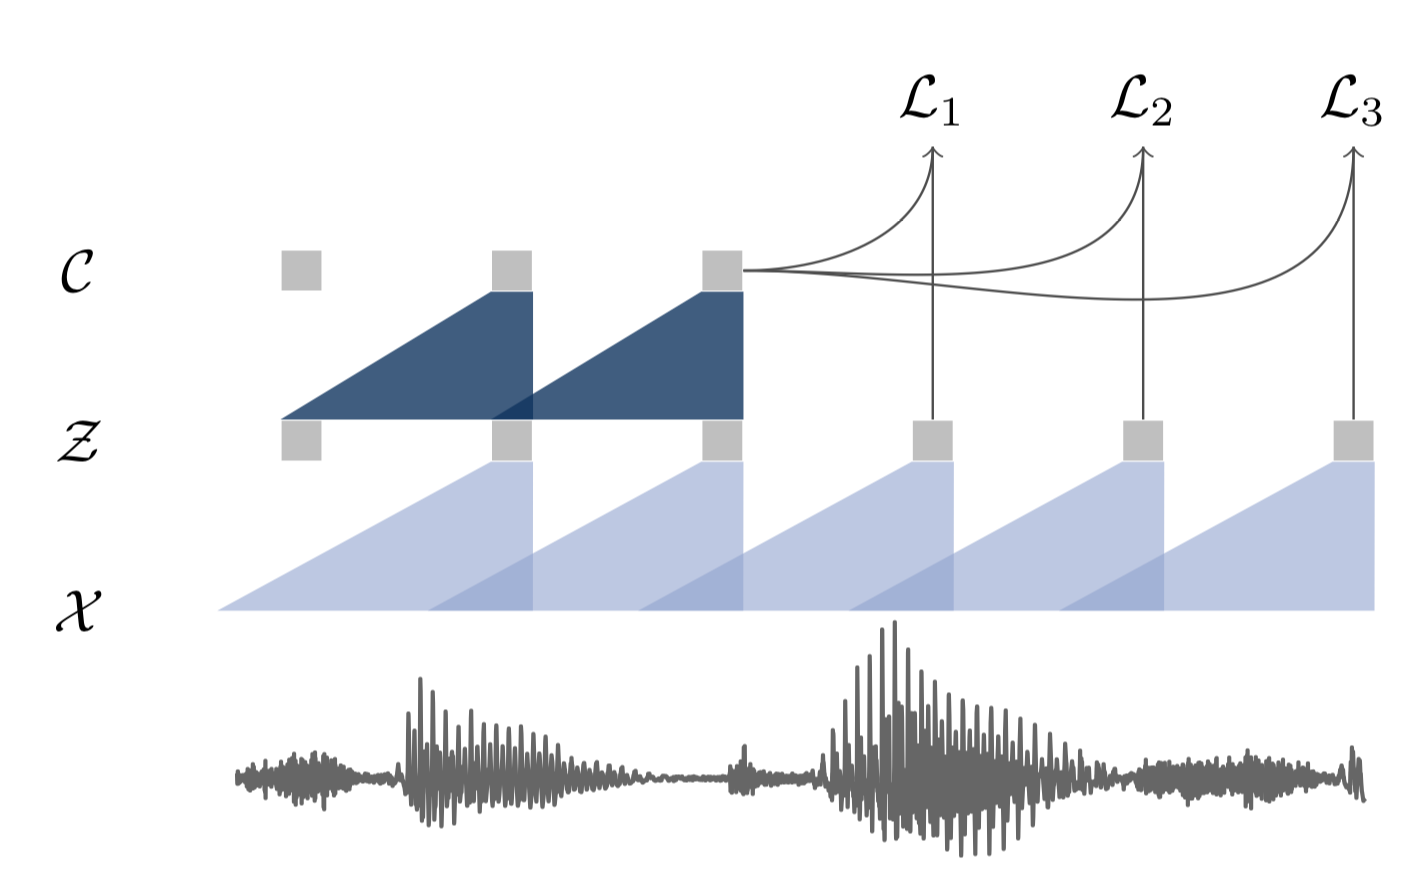
\includegraphics[scale=0.15]	{unsupervisedspeech.png} 
		%	[scale=0.35,trim=0mm 140mm 0mm 0mm,clip=true]
			\caption{Figure from \citep{DBLP:journals/corr/abs-1904-05862}}
			\label{fig:unsup}
			\end{figure}

	
\end{frame}

\begin{frame}
	\frametitle{Contrastive Predictive Coding (CPC)}
	Experiments
		\begin{itemize}
			\item After pre-training:  input the representations $c_i$ produced by the context network to the acoustic model instead of log-mel filterbank features
			\item ASR tasks: phoneme recognition on TIMIT and word recognition on WSJ
			\item Librispeech corpus (1000h) used for unsupervised pre-training
		\end{itemize} 


		\begin{figure}
			\centering
			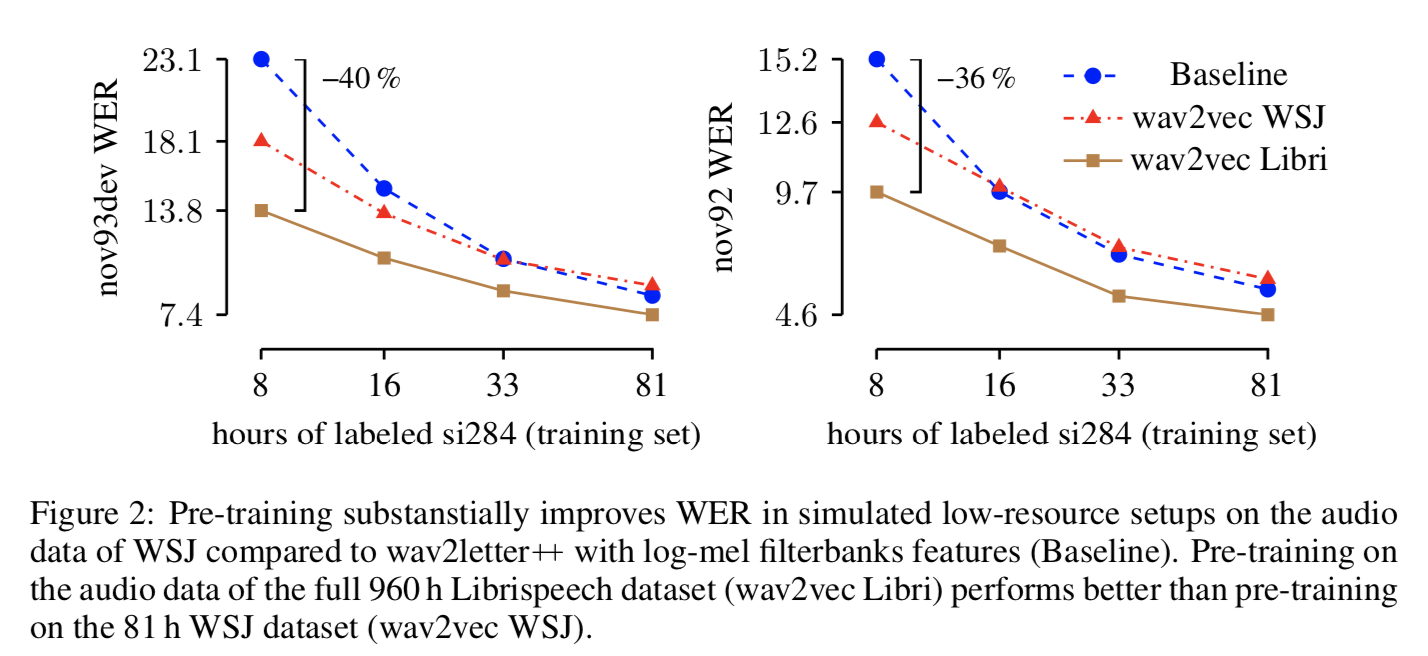
\includegraphics[scale=0.36]	{results.png} 
		%	[scale=0.35,trim=0mm 140mm 0mm 0mm,clip=true]
			\caption{Figure from \citep{DBLP:journals/corr/abs-1904-05862}}
			\label{fig:results}
			\end{figure}
	
\end{frame}


\begin{frame}
	\frametitle{Contrastive Predictive Coding (CPC)}
	Experiments
		\begin{itemize}
			\item Results on TIMIT (phone recognition)
			\item Focus on acoustic modeling
		\end{itemize} 


		\begin{figure}
			\centering
			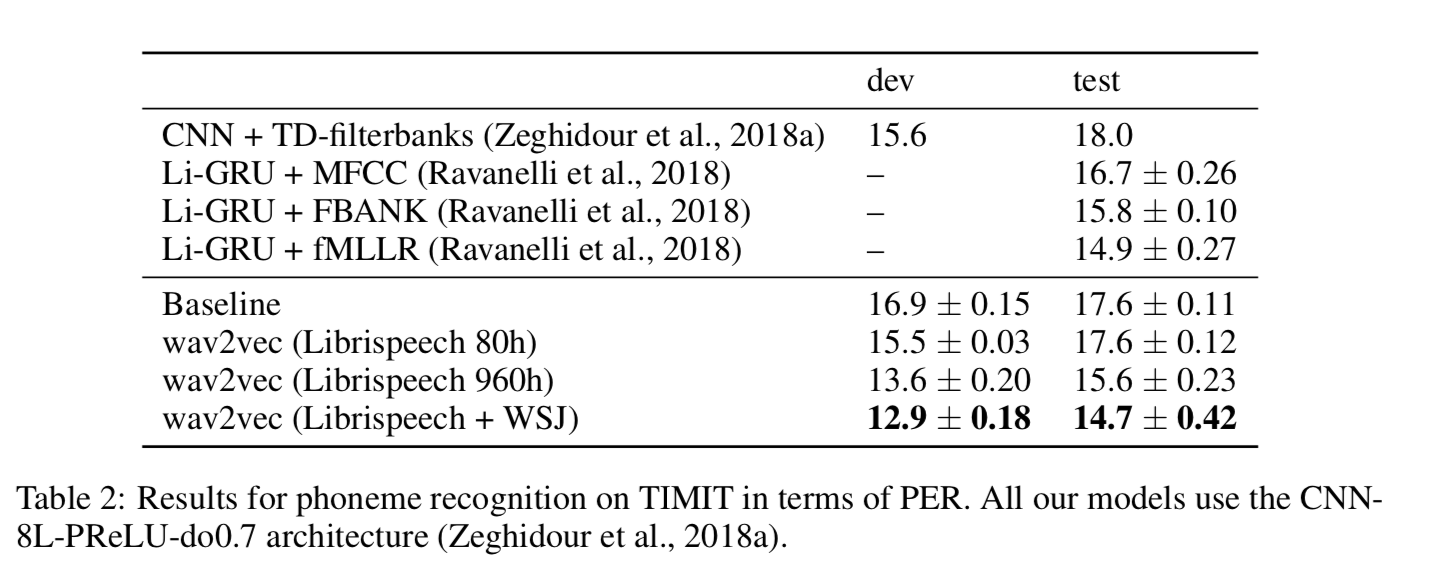
\includegraphics[scale=0.36]	{timit.png} 
		%	[scale=0.35,trim=0mm 140mm 0mm 0mm,clip=true]
			\caption{Figure from \citep{DBLP:journals/corr/abs-1904-05862}}
			\label{fig:results}
			\end{figure}
	
\end{frame}

\begin{frame}
	\frametitle{Contrastive Predictive Coding (CPC)}
	Take home message
		\begin{itemize}
			\item Experiments on WSJ show that this approach not only improves resource-poor setups but also settings where all WSJ training data is used
			\item More data for pre-training improves performances
			\item Could also be  used for other tasks (speech translation)
			\item Pre-trained model on English Librispeech made available\footnote{\url{https://github.com/pytorch/fairseq/tree/master/examples/wav2vec}}
			\item (I could not find details on pre-training time...)
		\end{itemize} 


	
\end{frame}






%%%%%%%
\section{Multiple self-supervised tasks}


\begin{frame}
\frametitle{Representation learning with multiple self-supervised tasks}
\begin{itemize}
\item Problem-agnostic speech encoder (PASE) \citep{pascual2019}
\item PASE+:  robust speech recognition in noisy and reverberant environments \citep{ravanelli2020multitask}
\end{itemize} 
\end{frame}

%%%%%%%

\begin{frame}
\frametitle{Problem-agnostic speech encoder (PASE)}
\begin{itemize}
\item Problem-agnostic speech encoder (PASE) \citep{pascual2019}
\item Jointly tackle multiple self-supervised tasks using an ensemble of neural networks that cooperate to discover good speech representations
\item Approach requires consensus across tasks, more likely to learn general, robust, and transferable features
\item Authors find that such representations outperform more traditional hand-crafted features in different speech classification tasks such as speaker identification, emotion classification, and  ASR
\end{itemize} 
\end{frame}

%%%%%%%


\begin{frame}
\frametitle{Problem-agnostic speech encoder (PASE)}

		\begin{itemize}
			\item Encoder: SincNet \citep{syncnet2018} + Convblocks (receptive field 150ms)
			\item Workers: one for each task (see next slide)
		\end{itemize} 


		\begin{figure}
			\centering
			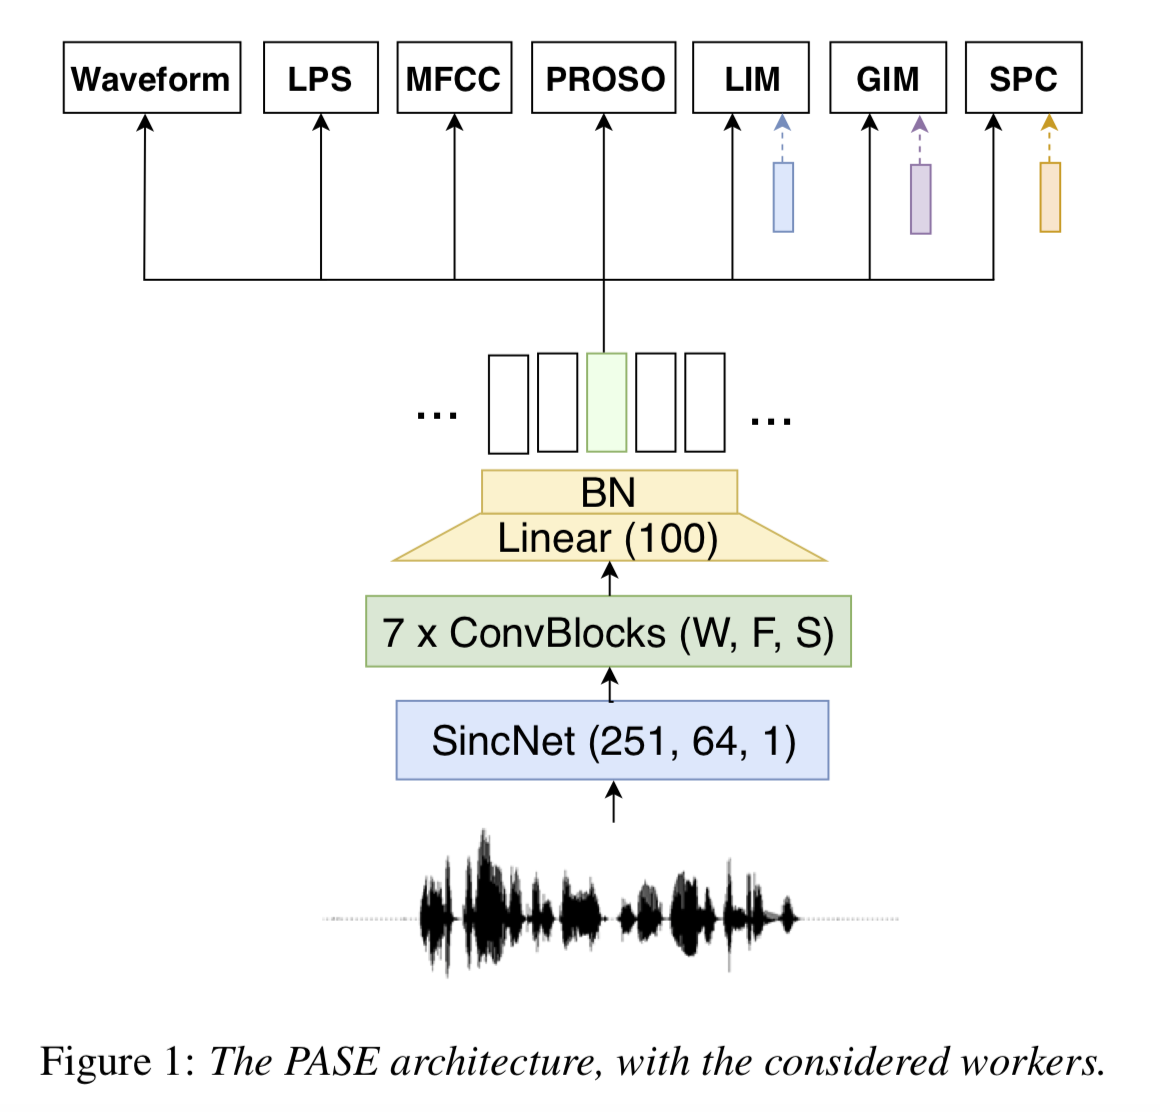
\includegraphics[scale=0.27]	{PASE} 
		%	[scale=0.35,trim=0mm 140mm 0mm 0mm,clip=true]
			\caption{Figure from \citep{pascual2019}}
			\end{figure}

\end{frame}

%%%%%%%

\begin{frame}
\frametitle{Problem-agnostic speech encoder (PASE)}

		\begin{itemize}
			\item Regression workers that solve 7 self-supervised tasks
			\item Trained to minimize the mean squared error (MSE) between the target features and the network predictions 
			\begin{itemize}
				\item \textbf{Waveform} learns to reconstruct waveforms
				\item \textbf{LPS} reconstruct log power spectrum 
				\item \textbf{MFCC} reconstruct  mel-frequency cepstral coefficients
				\item \textbf{Prosody} predicts 4 basic prosodic features per frame
				\item \textbf{LIM} (local info max) contrastive task where positive sample is drawn from the same utterance and a negative sample is drawn from another random utterance (that likely belongs to a different speaker)
				\item  \textbf{GIM} (global info max)  similar to LIM using global representations (averaged over 1s) instead of local ones
				\item \textbf{SPC} sequence predicting coding: similar to contrastive predictive coding (CPC) introduced earlier
			\end{itemize}
		\end{itemize} 




\end{frame}

%%%%%%%





\begin{frame}
\frametitle{Problem-agnostic speech encoder (PASE)}

		\begin{itemize}
			\item Experiments on speaker identification, emotion recognition and ASR
		\end{itemize} 


		\begin{figure}
			\centering
			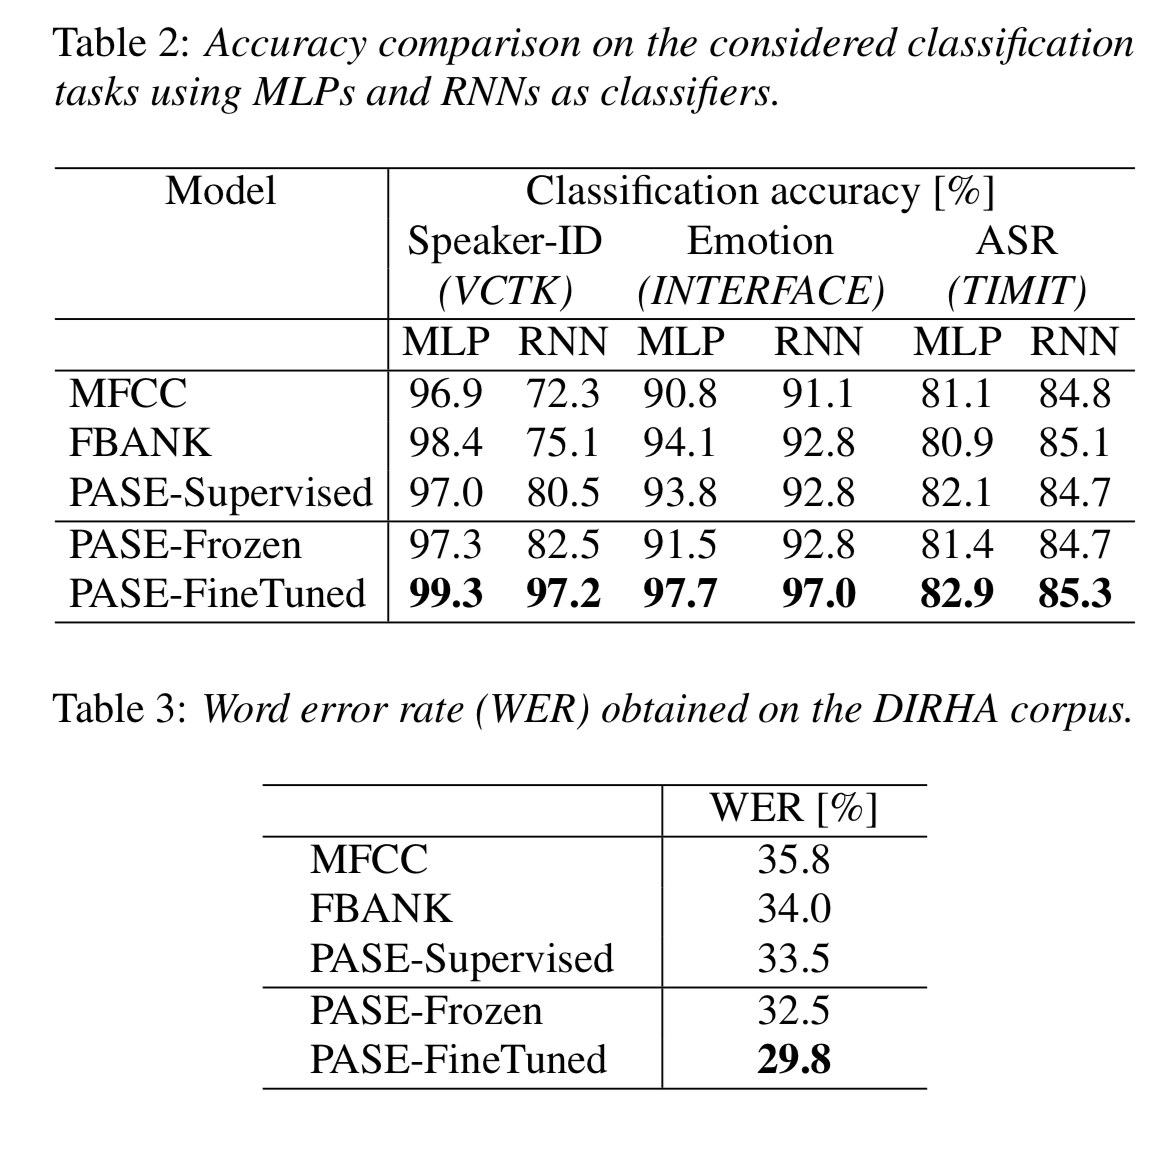
\includegraphics[scale=0.3]	{PASEexp} 
		%	[scale=0.35,trim=0mm 140mm 0mm 0mm,clip=true]
			\caption{Table from \citep{pascual2019}}
			\end{figure}

\end{frame}


\begin{frame}
\frametitle{PASE+:  Robust Speech Recognition in Noisy and Reverberant Environments}

		\begin{itemize}
			\item PASE+:  robust speech recognition in noisy and reverberant environments \citep{ravanelli2020multitask}
			\item Speech distortion to ''contaminate'' the input signals with a variety of random disturbances
		\end{itemize} 


		\begin{figure}
			\centering
			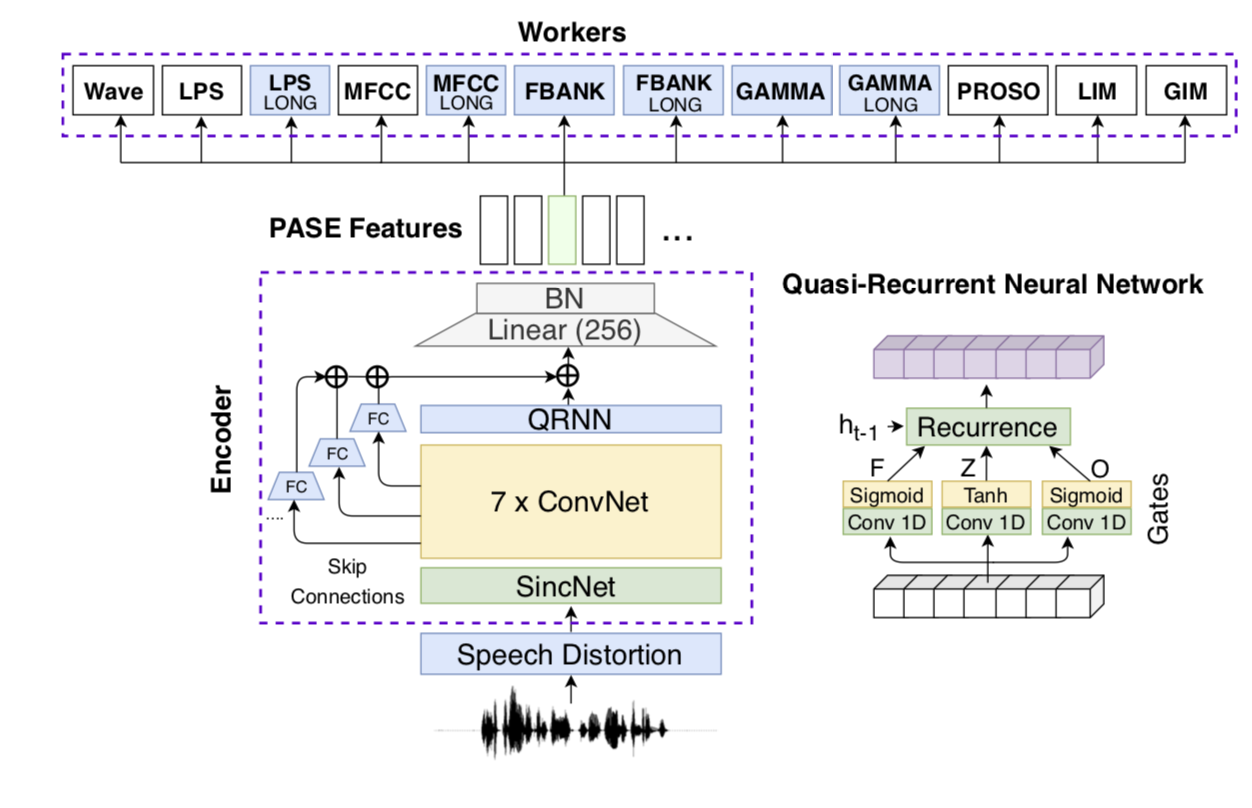
\includegraphics[scale=0.3]	{PASEplus} 
		%	[scale=0.35,trim=0mm 140mm 0mm 0mm,clip=true]
			\caption{Figure from \citep{ravanelli2020multitask}}
			\end{figure}

\end{frame}

\begin{frame}
\frametitle{PASE+:  Robust Speech Recognition in Noisy and Reverberant Environments}

		\begin{itemize}
			\item Different kinds of distorsions applied
		\end{itemize} 


		\begin{figure}
			\centering
			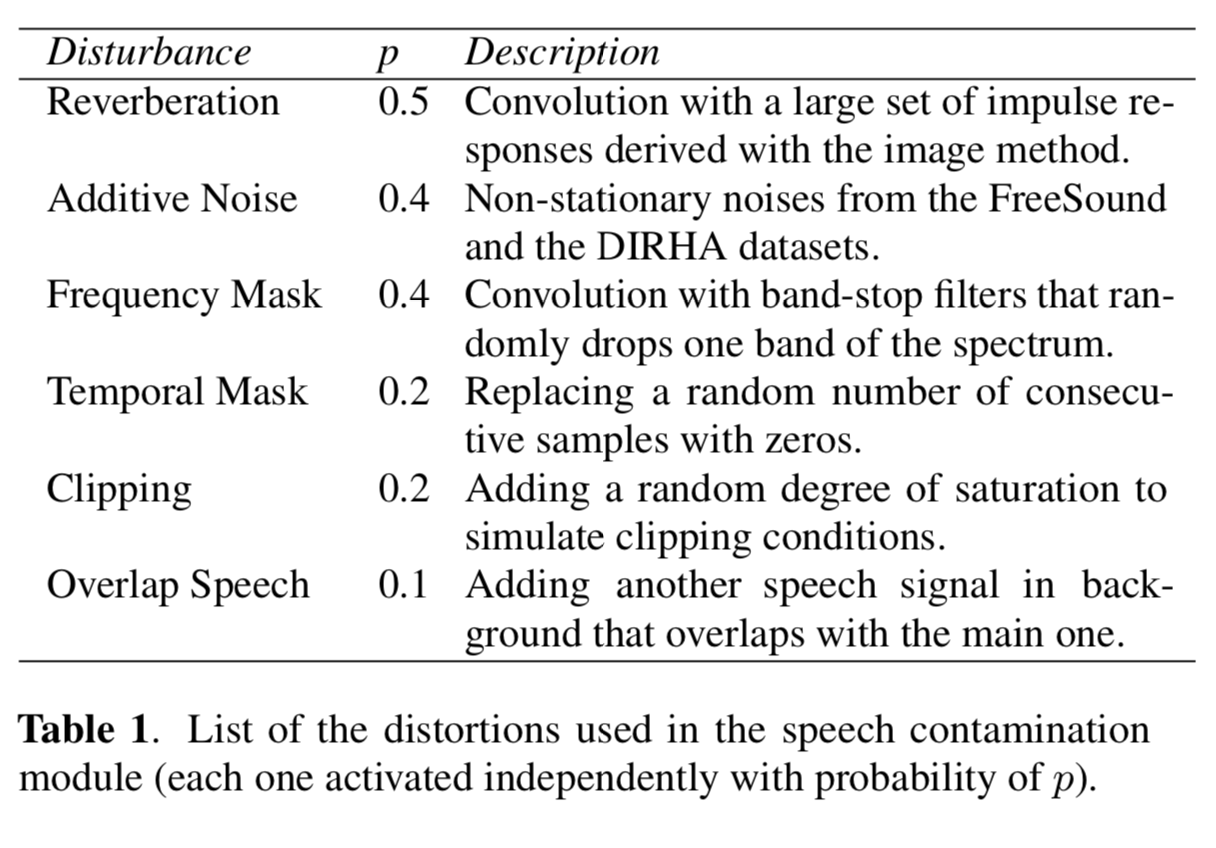
\includegraphics[scale=0.35]	{distorsions} 
		%	[scale=0.35,trim=0mm 140mm 0mm 0mm,clip=true]
			\caption{Table from \citep{ravanelli2020multitask}}
			\end{figure}

\end{frame}


\section{Encoder-decoder with bottleneck}


\begin{frame}
\frametitle{Unsupervised speech representation learning using WaveNet autoencoders \citep{DBLP:journals/corr/abs-1901-08810}}

		\begin{itemize}
			\item Learn latent representations that encode phonetic content only
			\item Rely on Wavnet decoder (used in TTS) to infer information that was rejected by the encoder
				\begin{itemize}
				\item acts as an inductive bias to allow encoder focusing on high level semantic features
				\end{itemize}
			\item Made up of 3 parts
				\begin{itemize}
				\item an encoder that computes a stream of latent vectors from speech input
				\item a bottleneck that encourages the encoder to discard portions of the latent representation which the decoder can recover
				\item a decoder which reconstructs the speech waveform 
				\end{itemize}			
		\end{itemize} 

\end{frame}



\begin{frame}
\frametitle{Unsupervised speech representation learning using WaveNet autoencoders}


		\begin{figure}
			\centering
			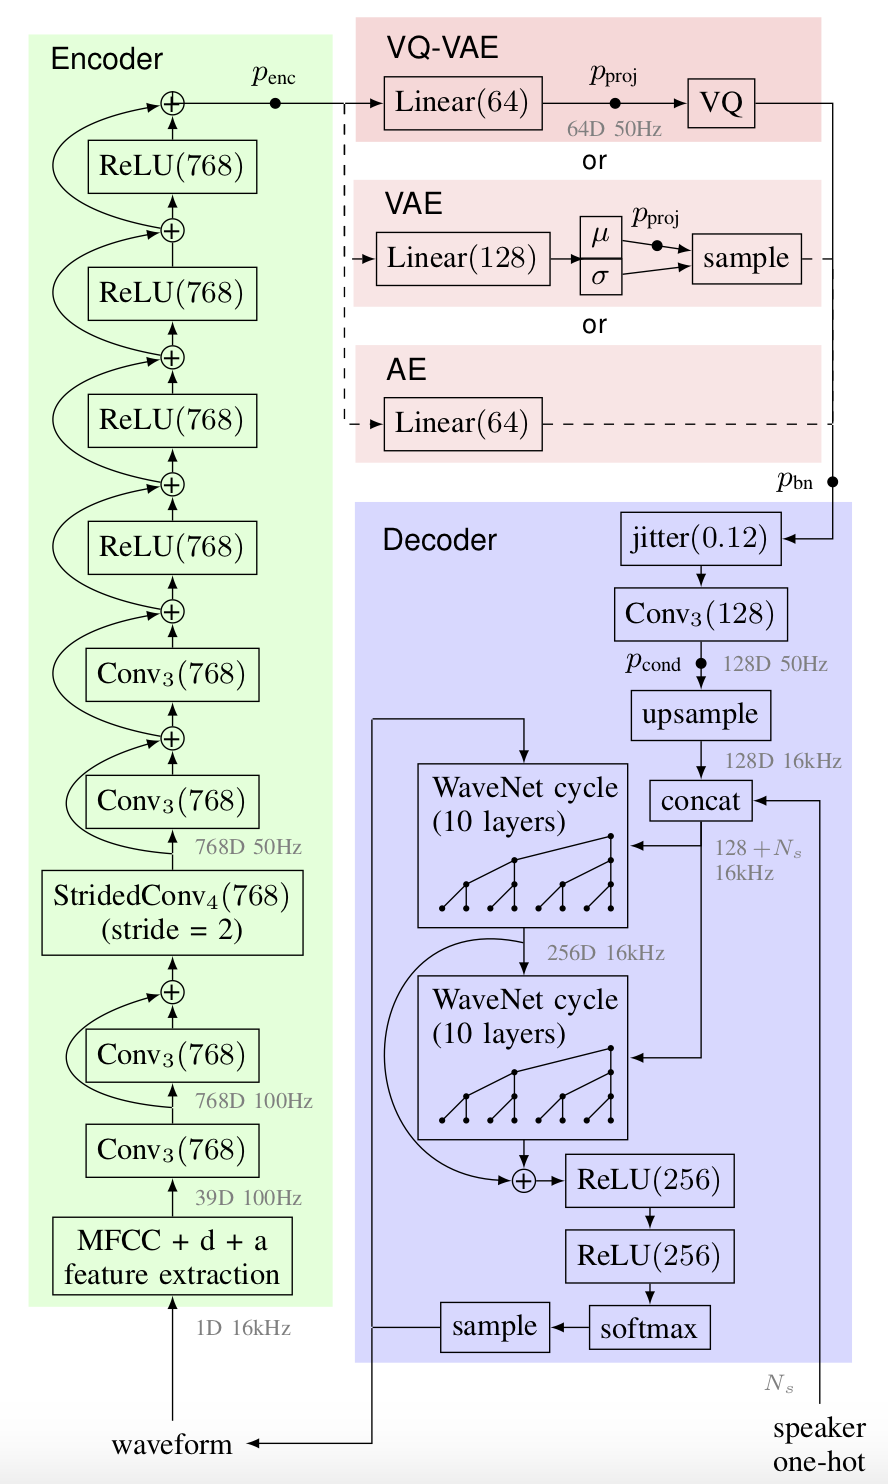
\includegraphics[scale=0.22]	{wavnetAE} 
		%	[scale=0.35,trim=0mm 140mm 0mm 0mm,clip=true]
			\caption{Figure from  \citep{DBLP:journals/corr/abs-1901-08810}}
			\end{figure}

\end{frame}


\begin{frame}
\frametitle{Unsupervised speech representation learning using WaveNet autoencoders}

		\begin{itemize}
			\item Three bottlneck variants are proposed
				\begin{itemize}
				\item a simple dimensionality reduction (AE)
				\item a Gaussian VAE with different latent representation dimensionalities and different capacities
				\item a VQ-VAE with different number of quantization prototypes 
				\end{itemize}		
			\item bottlenecks optionally followed by the dropout inspired time-jitter regularization	
				\begin{itemize}
				\item during training, each latent vector can replace either one or both of its neighbors
				\item promotes latent representation stability over time
				\end{itemize}			
		\end{itemize} 

\end{frame}

\begin{frame}
\frametitle{Unsupervised speech representation learning using WaveNet autoencoders}


		\begin{figure}
			\centering
			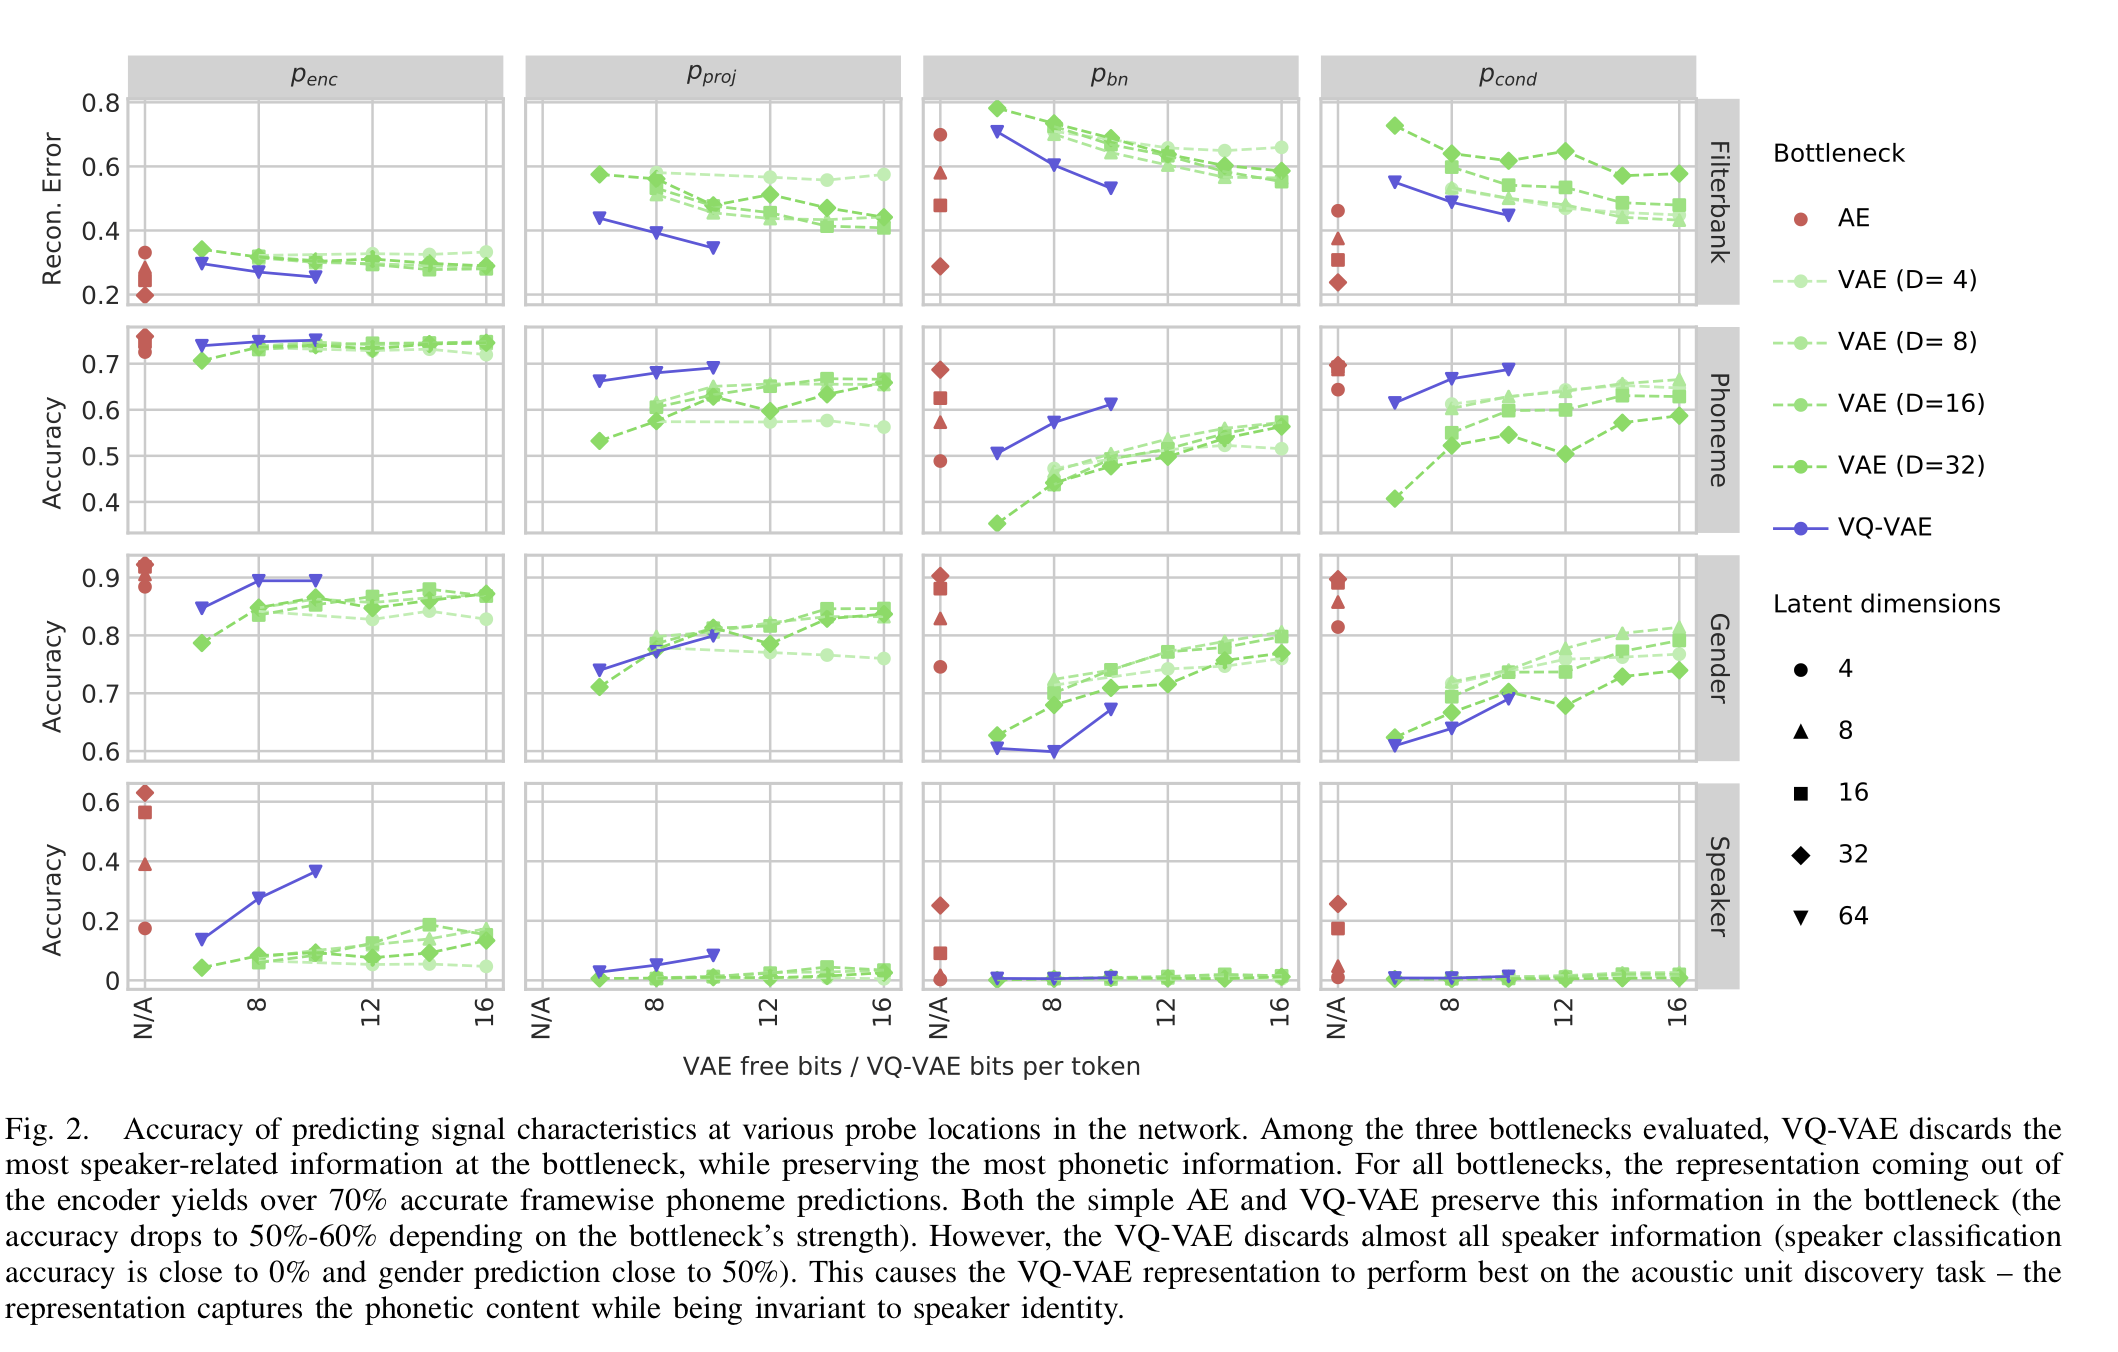
\includegraphics[scale=0.22]	{wavnetAEexp} 
		%	[scale=0.35,trim=0mm 140mm 0mm 0mm,clip=true]
			\caption{Table from  \citep{DBLP:journals/corr/abs-1901-08810}}
			\end{figure}

\end{frame}


\section{Beyond left-to-right (masked reconstruction)}

\begin{frame}
\frametitle{Beyond left-to-right}

		\begin{itemize}
			\item Speech-XLNet: Unsupervised Acoustic Model Pretraining For Self-Attention Networks \citep{song2019speechxlnet}
			\item Mockingjay: Unsupervised speech representation learning with deep bidirectional transformer encoders \citep{Liu_2020}
			\item Unsupervised pre-training of bidirectional speech encoders via masked reconstruction \citep{wang2020unsupervised}
		\end{itemize} 



\end{frame}


\begin{frame}
\frametitle{Speech-XLNet }

		\begin{itemize}
			\item Speech-XLNet \citep{song2019speechxlnet}
			\item Learn speech representations with self-attention networks 
			\item BERT-like autoencoding (AE) scheme to train a bi-directional speech representation model (not only left-to-right)
			\item Mask and reconstruct speech frames rather than word tokens (regression instead of classification task)
			\item Encourage network to learn global structures by shuffling speech frame orders (can be also seen as dynamic data augmentation)
			\item Training using a Mean Absolute Error (MAE) loss over several permutations of the input frames
		\end{itemize} 
\end{frame}


\begin{frame}
\frametitle{Speech-XLNet}

		\begin{itemize}
			\item Experiments on Hybrid and end-to-end ASR
			\item Results of Hybrid ASR on TIMIT are reported below
		\end{itemize} 


		\begin{figure}
			\centering
			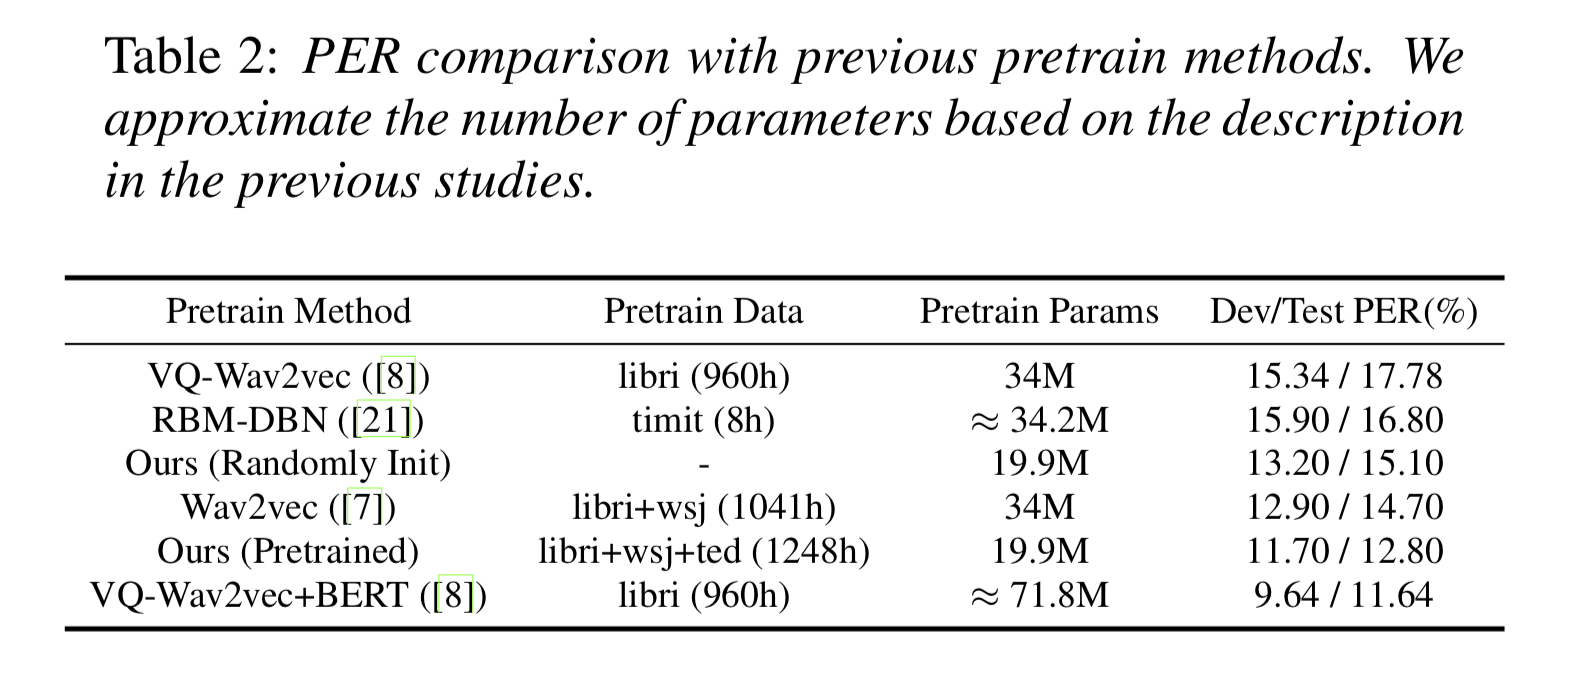
\includegraphics[scale=0.35]	{speechXLNETtable} 
		%	[scale=0.35,trim=0mm 140mm 0mm 0mm,clip=true]
			\caption{Table from  \citep{song2019speechxlnet}}
			\end{figure}

\end{frame}

\begin{frame}
\frametitle{Unsupervised speech representation learning with deep bidirectional transformer encoders}

		\begin{itemize}
			\item Predict the current frame through jointly conditioning on both past and future contexts (Mockingjay \citep{Liu_2020})
			\item Masked acoustic modeling task (rand. mask 15\% of input frames)\footnote{Use of additional consecutive masking where they mask consecutive frames $C_{num}$ to zero. The model is required to infer on global rather than local structure.}
			\item Use multi-layer transformer encoders and multi-head self-attention
			\item Add a prediction head (2 layers of feed-forward network with layer-norm) using last encoder layer as input
		\end{itemize} 
		
				\begin{figure}
			\centering
			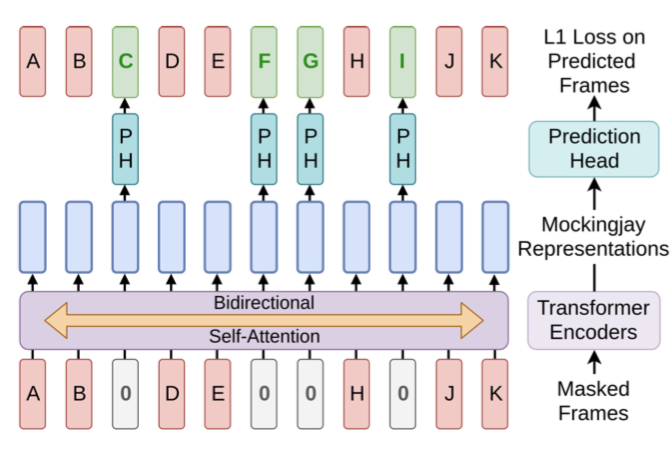
\includegraphics[scale=0.14]	{mockingjay} 
		%	[scale=0.35,trim=0mm 140mm 0mm 0mm,clip=true]
			\caption{Table from  \citep{Liu_2020}}
			\end{figure}


\end{frame}

\begin{frame}
\frametitle{Unsupervised speech representation learning with deep bidirectional transformer encoders}

		\begin{itemize}
			\item Experiments on phoneme classification
			\item With different amount of annotated data for training
		\end{itemize} 


		\begin{figure}
			\centering
			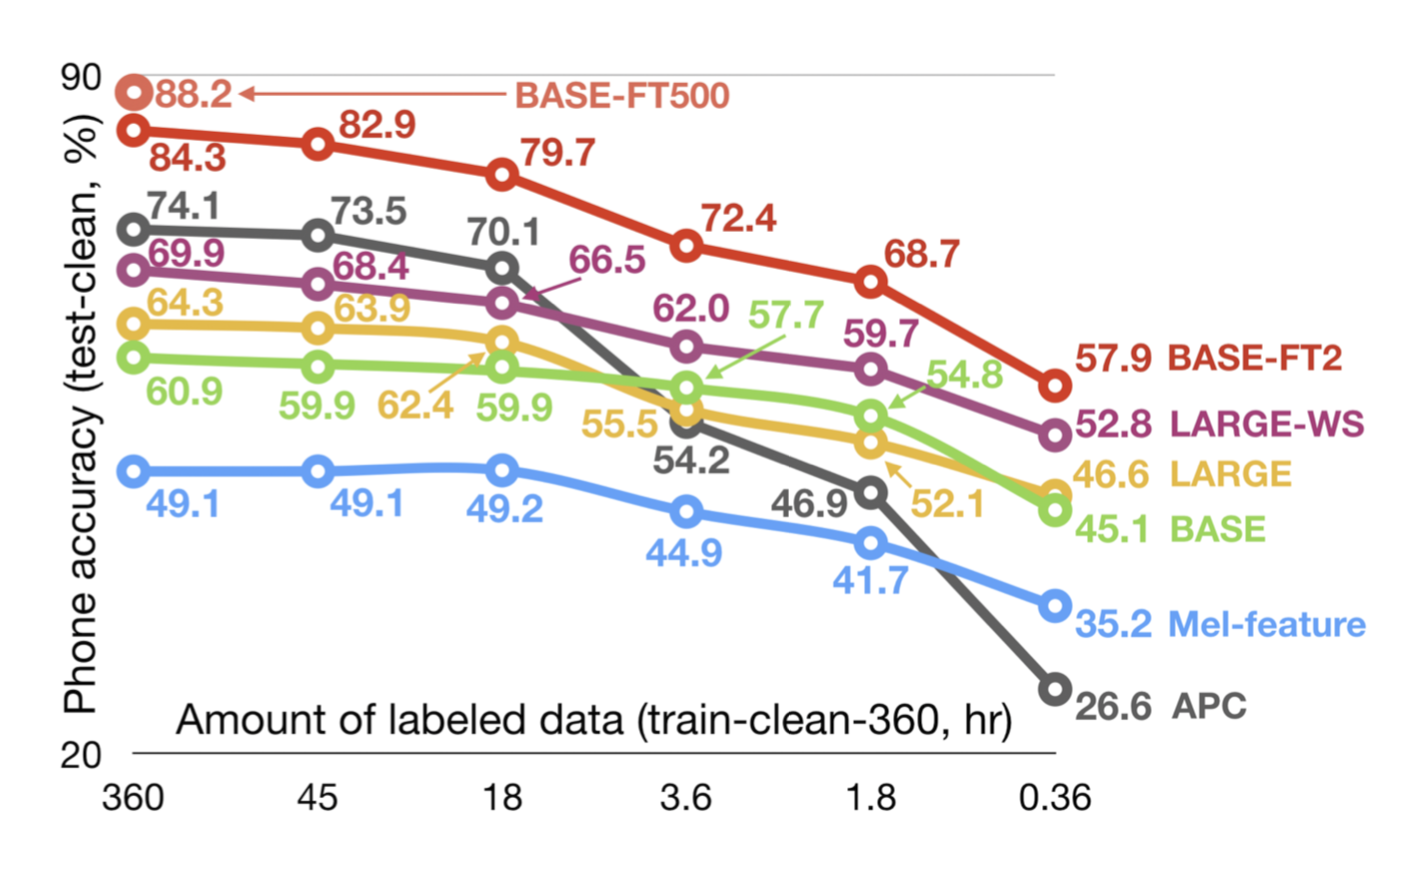
\includegraphics[scale=0.3]	{mockingjay-exp} 
		%	[scale=0.35,trim=0mm 140mm 0mm 0mm,clip=true]
			\caption{Figure from  \citep{Liu_2020}}
			\end{figure}

\end{frame}


\begin{frame}
\frametitle{Unsupervised Pre-training of Bidirectional Speech Encoders via Masked Reconstruction}

		\begin{itemize}
			\item Pre-training speech representations via a (BERT-style) masked reconstruction loss  \citep{wang2020unsupervised}
			\item Masking in both frequency and time to encourage model to exploit spatio-temporal info
			\item Elegant extension of data augmentation technique SpecAugment \citep{Park_2019}
		\end{itemize}	
			\begin{figure}
			\centering
			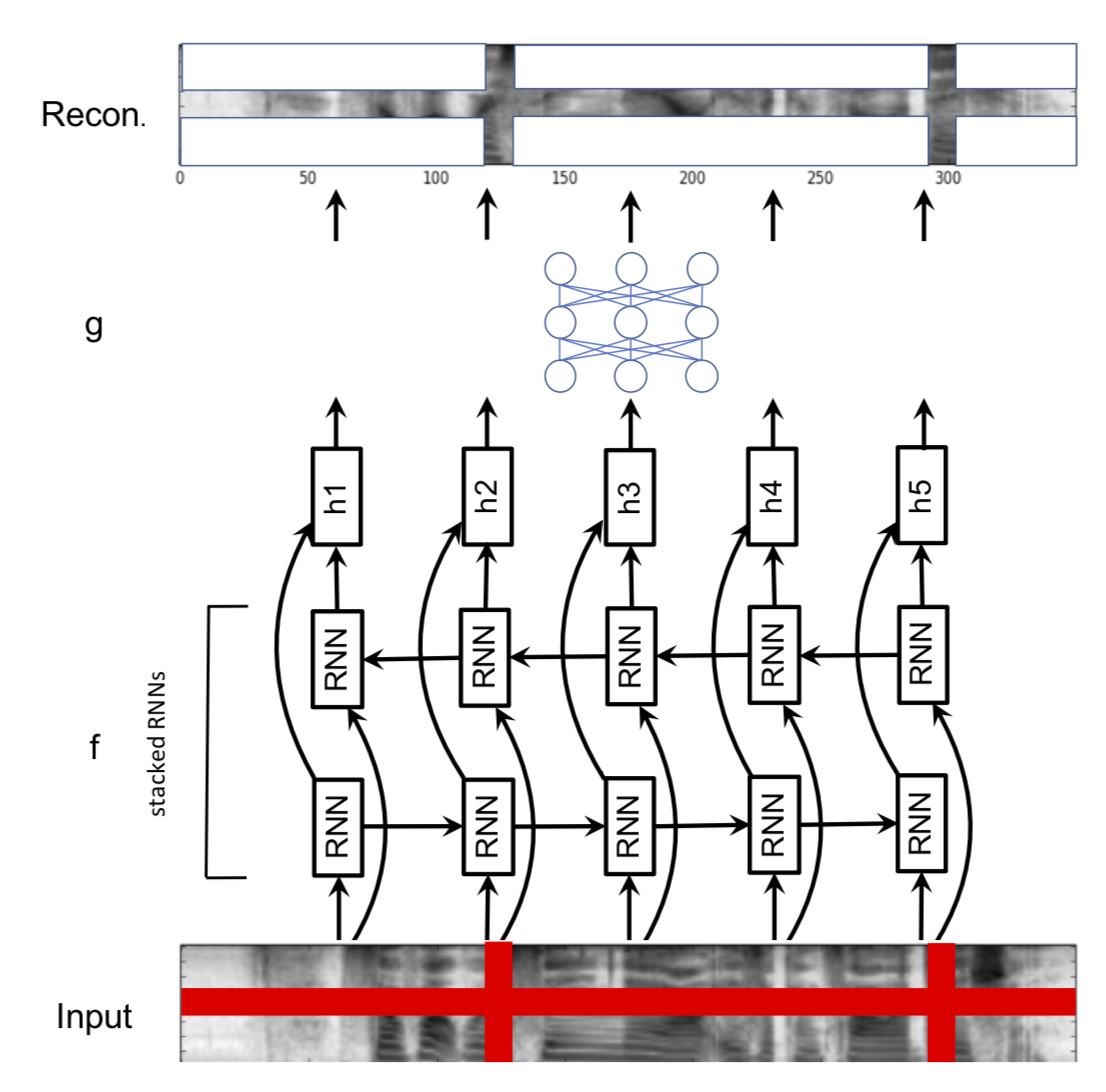
\includegraphics[scale=0.18]	{wang2020} 
		%	[scale=0.35,trim=0mm 140mm 0mm 0mm,clip=true]
			\caption{Figure from  \citep{wang2020unsupervised}}
			\end{figure}


\end{frame}


\begin{frame}
\frametitle{Unsupervised Pre-training of Bidirectional Speech Encoders via Masked Reconstruction}

	
		\begin{figure}
			\centering
			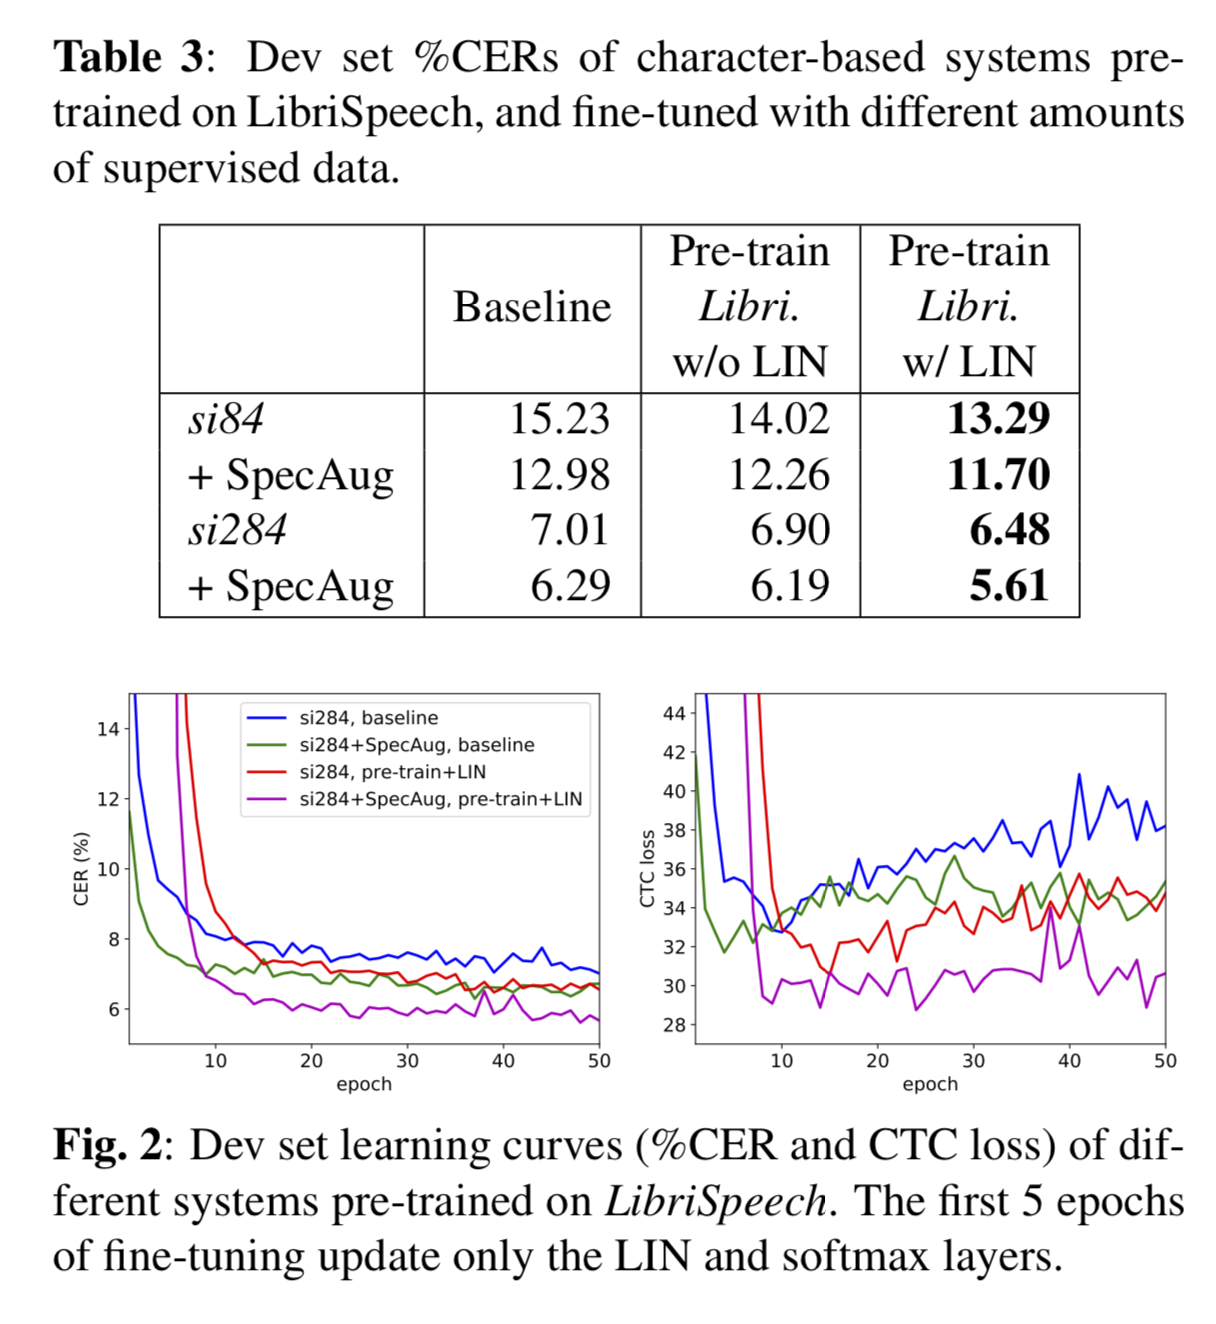
\includegraphics[scale=0.27]	{wang2020exp} 
		%	[scale=0.35,trim=0mm 140mm 0mm 0mm,clip=true]
			\caption{From  \citep{wang2020unsupervised}}
			\end{figure}

\end{frame}


\section{Probabilistic Latent Variable Models (LVMs)}

\begin{frame}
\frametitle{A Convolutional Deep Markov Model for Unsupervised Speech Representation Learning}

		\begin{itemize}
			\item A generative model for speech representation learning  \citep{khurana2020convolutional}
			\item Convolutional deep Markov model (ConvDMM)\footnote{Read \url{https://arxiv.org/pdf/2006.02547.pdf} for more details!}
			\item A Gaussian state-space model with non-linear emission and transition functions modelled by deep neural networks
			\item Directly based on the Deep Markov Model proposed by \citep{krishnan2016structured}
			\item Outperform multiple self-supervised methods on ASR and is complementary with self-supervised methods like Wav2Vec and PASE
		\end{itemize}

\end{frame}



\section{Exemple of application for translation of un-transcribed  speech}

\begin{frame}
\frametitle{Application to Speech Translation in Low Resource Conditions (submitted to IS2020)}

		\begin{itemize}
			\item Investigate the possibility to leverage unlabeled speech for end-to-end automatic speech translation (AST)
			\item We focus on scenarios where 
				\begin{itemize}
					\item (a) recordings in source language are not transcribed\footnote{Transcription not available or language poorly written} (no ASR pre-training is possible), 
					\item (b) only a small-medium amount of training data (speech aligned to translations) is available, 
					\item (c) a larger amount of unlabeled speech can be used. 			
				\end{itemize}
			\item Scenario typical of situations when one builds a system that translates from speech in a language with poorly standardized orthography or even from an unwritten language
		\end{itemize}

\end{frame}


\begin{frame}
\frametitle{Application to Speech Translation in Low Resource Conditions (submitted to IS2020)}

		\begin{itemize}
			\item Speech translation experiments on How2 En-Pt corpus
			\item Fbank versus Wav2Vec features
			\item Impact of fine tuning Wav2Vec model on untranscribed speech 
			\item Self supervised representations have strong impact in low resource conditions
			\item Validation on other language pairs (en-fr and en-de) confirm this trend
			\end{itemize}

	\begin{figure}
			\centering
			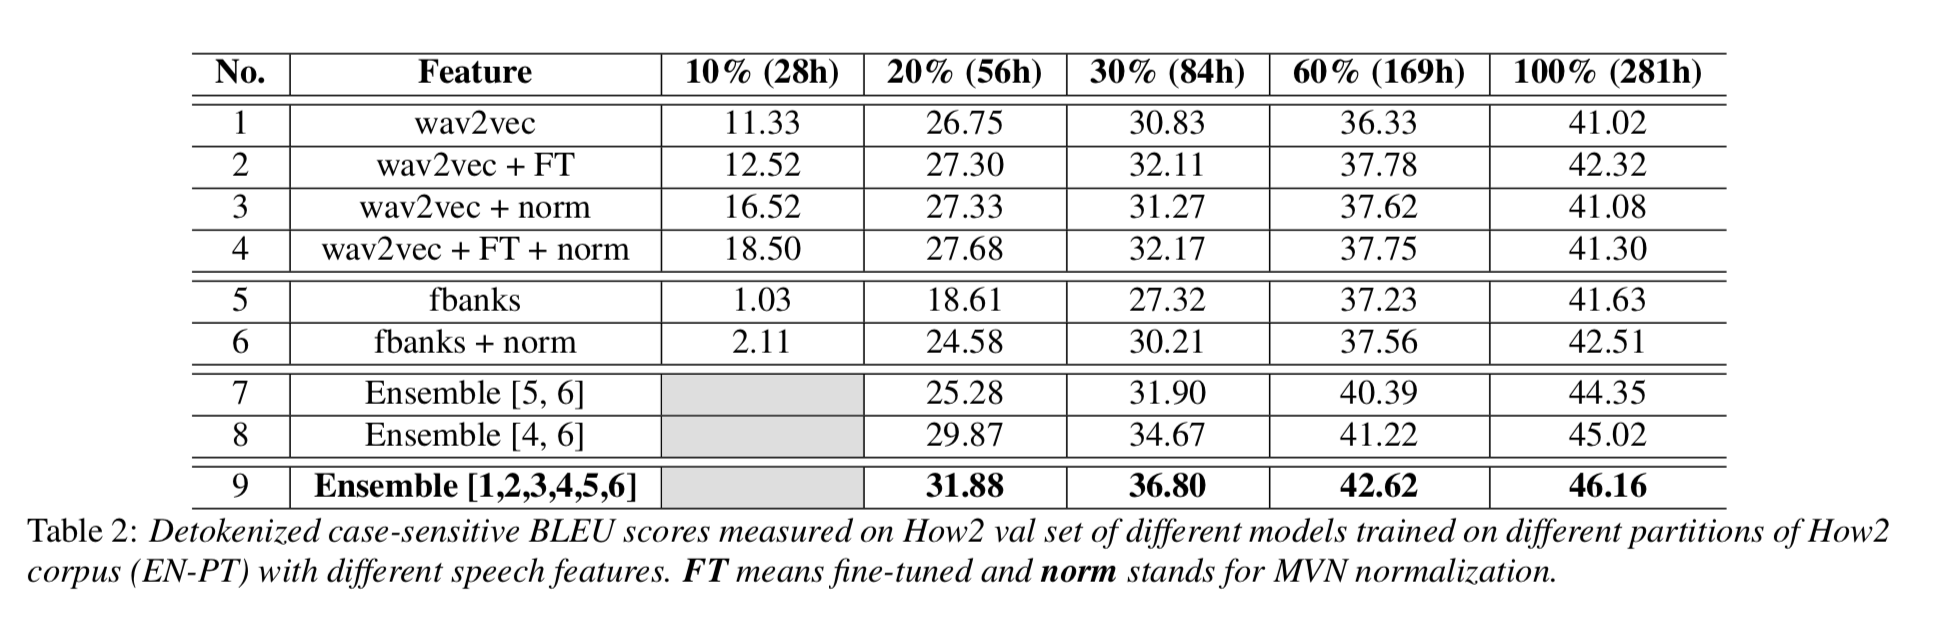
\includegraphics[scale=0.27]	{how2ast} 
		%	[scale=0.35,trim=0mm 140mm 0mm 0mm,clip=true]
			\end{figure}



\end{frame}


\section{Takeaways}



\begin{frame}
\frametitle{Takeaways}

		\begin{itemize}
			\item Self-supervised representation learning from speech using future or past-future context
			\item Allows to adopt the pre-training + fine tuning methodology widely used in (text) NLP 
			\item Reduce dependence on labeled data for building speech systems (speech transcription, translation, paralinguistics)
			\item Particularly efficient in low resource scenarios (few annotated data)
			\item A rapidly evolving sub-domain (from APC/CPC to masked reconstruction models) 
			\item Very recent approaches based on generative models \citep{khurana2020convolutional}
			\item \textbf{Not shared benchmark to evaluate all these approaches} - need something equivalent to GLUE/SuperGLUE in NLP !!
		\end{itemize}
\end{frame}







%%%%%%%

%%%%%%%





\begin{frame}
	\frametitle{Questions?}
	
	\vfill
	\centerline{\Huge Thank you}
	\vfill
\end{frame}







%_______________________________________________________





\begin{frame}[allowframebreaks]
        \frametitle{References}
        {\scriptsize
        \bibliographystyle{apalike}
        \bibliography{laurent,mybib,refs}}
\end{frame}    





\end{document}







